%%%%%%%%%%%%%%%%%%%%%%%%%%%%%%%%%%%%%%%%%
% Masters/Doctoral Thesis 
% LaTeX Template
% Version 1.42 (19/1/14)
%
% This template has been downloaded from:
% http://www.latextemplates.com
%
% Original authors:
% Steven Gunn 
% http://users.ecs.soton.ac.uk/srg/softwaretools/document/templates/
% and
% Sunil Patel
% http://www.sunilpatel.co.uk/thesis-template/
%
% License:
% CC BY-NC-SA 3.0 (http://creativecommons.org/licenses/by-nc-sa/3.0/)
%
% Note:
% Make sure to edit document variables in the Thesis.cls file
%
%%%%%%%%%%%%%%%%%%%%%%%%%%%%%%%%%%%%%%%%%

%----------------------------------------------------------------------------------------
%	PACKAGES AND OTHER DOCUMENT CONFIGURATIONS
%----------------------------------------------------------------------------------------

\documentclass[11pt, a4paper, oneside]{Thesis} % Paper size, default font size and one-sided paper

\graphicspath{{Pictures/}} % Specifies the directory where pictures are stored

\usepackage[square, numbers, comma, sort&compress]{natbib} % Use the natbib reference package - read up on this to edit the reference style; if you want text (e.g. Smith et al., 2012) for the in-text references (instead of numbers), remove 'numbers' 
\hypersetup{urlcolor=blue, colorlinks=true} % Colors hyperlinks in blue - change to black if annoying
\title{\ttitle} % Defines the thesis title - don't touch this

% added package for algortihm in IEEE default style
\usepackage{algorithmic}
\usepackage{algorithm}
\begin{document}

\frontmatter % Use roman page numbering style (i, ii, iii, iv...) for the pre-content pages

\setstretch{1.3} % Line spacing of 1.3

% Define the page headers using the FancyHdr package and set up for one-sided printing
\fancyhead{} % Clears all page headers and footers
\rhead{\thepage} % Sets the right side header to show the page number
\lhead{} % Clears the left side page header

\pagestyle{fancy} % Finally, use the "fancy" page style to implement the FancyHdr headers

\newcommand{\HRule}{\rule{\linewidth}{0.5mm}} % New command to make the lines in the title page

% PDF meta-data
\hypersetup{pdftitle={\ttitle}}
\hypersetup{pdfsubject=\subjectname}
\hypersetup{pdfauthor=\authornames}
\hypersetup{pdfkeywords=\keywordnames}

%----------------------------------------------------------------------------------------
%	TITLE PAGE
%----------------------------------------------------------------------------------------

\begin{titlepage}
\begin{center}

\textsc{\LARGE \univname}\\[1.5cm] % University name
\textsc{\Large Master's Thesis}\\[0.5cm] % Thesis type

\HRule \\[0.4cm] % Horizontal line
{\huge \bfseries \ttitle}\\[0.4cm] % Thesis title
\HRule \\[1.5cm] % Horizontal line
 
\begin{minipage}{0.4\textwidth}
\begin{flushleft} \large
\emph{Author:}\\
\href{https://github.com/debajyoti7/}{\authornames} % Author name - remove the \href bracket to remove the link
\end{flushleft}
\end{minipage}
\begin{minipage}{0.4\textwidth}
\begin{flushright} \large
\emph{Supervisor:} \\
\href{http://www.es.mdh.se/staff/15-Baran_____r__kl__}{\supname} % Supervisor name - remove the \href bracket to remove the link  
\end{flushright}
\end{minipage}\\[3cm]
 
\large \textit{A thesis submitted in fulfilment of the requirements\\ for the degree of \degreename}\\[0.3cm] % University requirement text
\textit{in the}\\[0.4cm]
\groupname\\\deptname\\[2cm] % Research group name and department name
 
{\large \today}\\[4cm] % Date
%\includegraphics{Logo} % University/department logo - uncomment to place it
 
\vfill
\end{center}

\end{titlepage}

%----------------------------------------------------------------------------------------
%	DECLARATION PAGE
%	Your institution may give you a different text to place here
%----------------------------------------------------------------------------------------

\Declaration{

\addtocontents{toc}{\vspace{1em}} % Add a gap in the Contents, for aesthetics

I, \authornames, declare that this thesis titled, '\ttitle' and the work presented in it are my own. I confirm that:

\begin{itemize} 
\item[\tiny{$\blacksquare$}] This work was done wholly or mainly while in candidature for a research degree at this University.
\item[\tiny{$\blacksquare$}] Where any part of this thesis has previously been submitted for a degree or any other qualification at this University or any other institution, this has been clearly stated.
\item[\tiny{$\blacksquare$}] Where I have consulted the published work of others, this is always clearly attributed.
\item[\tiny{$\blacksquare$}] Where I have quoted from the work of others, the source is always given. With the exception of such quotations, this thesis is entirely my own work.
\item[\tiny{$\blacksquare$}] I have acknowledged all main sources of help.
\item[\tiny{$\blacksquare$}] Where the thesis is based on work done by myself jointly with others, I have made clear exactly what was done by others and what I have contributed myself.\\
\end{itemize}
 
Signed:\\
\rule[1em]{25em}{0.5pt} % This prints a line for the signature
 
Date:\\
\rule[1em]{25em}{0.5pt} % This prints a line to write the date
}

\clearpage % Start a new page

%----------------------------------------------------------------------------------------
%	QUOTATION PAGE
%----------------------------------------------------------------------------------------

\pagestyle{empty} % No headers or footers for the following pages

\null\vfill % Add some space to move the quote down the page a bit
\begin{center}
\textit{``Knowledge is the food of the soul."}
\end{center}

\begin{flushright}
Plato.
\end{flushright}

\vfill\vfill\vfill\vfill\vfill\vfill\null % Add some space at the bottom to position the quote just right

\clearpage % Start a new page

%----------------------------------------------------------------------------------------
%	ABSTRACT PAGE
%----------------------------------------------------------------------------------------

\addtotoc{Abstract} % Add the "Abstract" page entry to the Contents

\abstract{\addtocontents{toc}{\vspace{1em}} % Add a gap in the Contents, for aesthetics

There is a dire need of understanding the inner workings in of a social structure to fully utilize the potential of the connections. This thesis aims at analyzing different policies for spread of an idea in the society, to gain insight into methods to strike a balance in utility and cost incurred for the same.
}

\clearpage % Start a new page

%----------------------------------------------------------------------------------------
%	ACKNOWLEDGEMENTS
%----------------------------------------------------------------------------------------

\setstretch{1.3} % Reset the line-spacing to 1.3 for body text (if it has changed)

\acknowledgements{\addtocontents{toc}{\vspace{1em}} % Add a gap in the Contents, for aesthetics
\begin{center}
Thanks to Baran for the valuable guidance and patience.

Thanks to Carina for her guidance regarding the aspects of Innovation Management.

Thanks to my loved ones for their support and encouragement.
\end{center}
}
\clearpage % Start a new page

%----------------------------------------------------------------------------------------
%	LIST OF CONTENTS/FIGURES/TABLES PAGES
%----------------------------------------------------------------------------------------

\pagestyle{fancy} % The page style headers have been "empty" all this time, now use the "fancy" headers as defined before to bring them back

\lhead{\emph{Contents}} % Set the left side page header to "Contents"
\tableofcontents % Write out the Table of Contents

\lhead{\emph{List of Figures}} % Set the left side page header to "List of Figures"
\listoffigures % Write out the List of Figures

\lhead{\emph{List of Tables}} % Set the left side page header to "List of Tables"
\listoftables % Write out the List of Tables

%----------------------------------------------------------------------------------------
%	ABBREVIATIONS
%----------------------------------------------------------------------------------------

\clearpage % Start a new page

\setstretch{1.5} % Set the line spacing to 1.5, this makes the following tables easier to read

\lhead{\emph{Abbreviations}} % Set the left side page header to "Abbreviations"
\listofsymbols{ll} % Include a list of Abbreviations (a table of two columns)
{
%\textbf{Acronym} & \textbf{W}hat (it) \textbf{S}tands \textbf{F}or \\
\textbf{BA} & \textbf{B}arabási \textbf{A}lbert model \\
\textbf{CG} & \textbf{C}ontinuous \textbf{G}rowth \\
\textbf{PA} & \textbf{P}referential \textbf{A}ttachment \\
\textbf{CPS} & \textbf{C}yber \textbf{P}hysical \textbf{S}ystems \\
\textbf{M2M} & \textbf{M}achine to \textbf{M}achine \\
\textbf{IoT} &	\textbf{I}nternet of \textbf{T}hingss \\
}


%----------------------------------------------------------------------------------------
%	DEDICATION
%----------------------------------------------------------------------------------------

\setstretch{1.3} % Return the line spacing back to 1.3

\pagestyle{empty} % Page style needs to be empty for this page

\dedicatory{For the bewildered spirits who make it their business to know that which other men don't.} % Dedication text

\addtocontents{toc}{\vspace{2em}} % Add a gap in the Contents, for aesthetics

%----------------------------------------------------------------------------------------
%	THESIS CONTENT - CHAPTERS
%----------------------------------------------------------------------------------------

\mainmatter % Begin numeric (1,2,3...) page numbering

\pagestyle{fancy} % Return the page headers back to the "fancy" style

% Include the chapters of the thesis as separate files from the Chapters folder
% Uncomment the lines as you write the chapters

% Chapter 1

\chapter{Introduction} % Main chapter title

\label{Chapter1} % For referencing the chapter elsewhere, use \ref{Chapter1} 

\lhead{Chapter 1. \emph{Introduction to the thesis}} % This is for the header on each page - perhaps a shortened title

%----------------------------------------------------------------------------------------

\section{Networks}
A network is an arrangement of two or more different entities, mostly linked together for sharing resources. The resources being shared can be either physical or otherwise. These entities being connected are referred to as nodes, and the links between them are called the connections of the network. 

\subsection{Computer Networks}
Computer Networks are networks of interconnected devices that can exchange and share information and resources. The nodes in a computer network can be devices such as laptop computers, smartphones, or even fitness trackers and smart wearables. These networks may be categorized depending on the type of connections being formed, and the rules or protocols governing communications between different nodes within the network. While most nodes may support both incoming and outgoing connections, some nodes may have restrictions and only support one type of connections. Such networks are also known as \textit{Data Networks}. 

\subsection{Social Networks}
Social Networks refer to arrangement of individual agents, most commonly humans or their digital representatives, such that these arrangements are dependent on the actions of the agents and also influence their future actions. This is also referred to as a `social structure'. With the personalization of technology, computer networks are shaping themselves to get even closer to the social networks in terms of structure, shape, size, and degree distribution, for example. A comprehensive review of the same was done by Newman~\cite{Newman03thestructure}. 

This is particularly important and interesting with the emergence of personalized wearable devices. This could lead to a 1:1 man to machine ratio, which would mean, when allowed, the personal devices would network exactly as their users.

\subsection{Scale-Free Networks}
A scale-free network is a network with the property that the fraction P(k) of nodes with `k' connections  is determined as: 

\begin{equation}
P(k) \sim k^{-\gamma}
\label{eqn:power law}
\end{equation}

In general, the degree distribution of the network follows a power law. This means that the network is scalable, and the properties of degree distribution of the nodes is not affected by the size of the network. These networks follow a strategy such that there are a lot of nodes with few connections, and a very few nodes with significantly larger number of connections. These highly-connected nodes can be thought of as hubs in the network.

The work in~\cite{1999Sci...286..509B} explains how diverse systems are best described as complex topological networks, and shows how prevalent scale-free networks are in natural as well as man-made structures alike. It presents a reproducible model which indicates strong self-governing principles lead to formation of such networks without being affected by the particulars of the individuals.

The author uses this approach successfully in this thesis to develop a model despite the heterogeneous nature of the different agents in the network.

\subsection{Innovation Diffusion}
\textit{Diffusion of innovations} refers to the theory of understanding the factors governing spread and acceptance of any new idea or product in a social system. It tries to understand and formalise the critical point in the process of spreading the idea after which the idea can self-sustain in the system. In his book~\cite{DiffusionofInnovations}, Everett Rogers explains how this process relies heavily on human capital and proposes the four main influencing factors, namely : 
\begin{tabular}{l}
\textit{The innovation itself} \\ 
\textit{Communication channels} \\ 
\textit{Time}, and \\ 
\textit{Social system} \\
\end{tabular} 

Among these, the author decided to focus on the effect of the structure of the social system and time of campaigning for this thesis. He also decided to restrict the communication channel as much as possible to accommodate for the fact of randomness and chance in real world scenarios.

\section{State of the Art}
Humans in present day society must network to sustain and complete tasks. Studies have shown networks to evolve over time to optimize functionalities, and increase reach and longevity. These evolutions may be guided or self-governed. The most coveted type of network, perhaps, is the kind formed naturally among varied entities, i.e., free scaling networks ~\cite{1999Sci...286..509B, 2002RvMP...74...47A}.

The first model for free scaling networks was proposed by Barab{\'a}si–Albert~\cite{1999Sci...286..509B}, hereinafter referred to as B-A model, and the works of Erd\H{o}s \& R\'{e}nyi~\cite{Erdos60onthe}, Watts and Strogatz~\cite{1251797}, Watts, Strogatz and Newman~\cite{PhysRevE.64.026118},  Saramäki  and Kaski~\cite{Saramaki200480} , Yang and Jure~\cite{Yang_modelinginformation} , and  Rycroft~\cite{Rycroft2007565} also helped greatly in laying the groundwork.

It is prominent that existing social networks tend to scale freely and it is safe to assume that personalized devices, if and when allowed to network, will follow a similar trace.

\subsection{State of the art in networked devices}

Internet of Things~\cite{Internet-of-things} - Internet connectivity and accessibility in present day enables direct linking of everyday physical objects, overcoming the spatio-temporal boundaries. This upgrades a part of our lives to the cloud and allows better incorporation of virtual reality in everyday life.
It makes our lives easier, but also raises confusion as the complexity of processes increases manifold. 

Cyber-Physical Systems and Machine-to-Machine~\cite{6601317} - Internet of Things is a small part of a larger picture, where computational devices of all size and shape interact with each other and with everyday objects to perform complex tasks, ranging from temperature control in a modern house, to automatic detection of outbreak of a potentially fatal epidemic.
Machine-to-Machine communication makes it possible for sensors spread over a large area to share the load of detecting varied signals, while some entirely different processing entity looks into that raw data and extracts meaningful information from it, and then a separate link actuates some physical entity to act based on the information just gathered. However, large scale implementations of Cyber-Physical Systems face a major challenge due to the heterogeneous nature of network elements.

\subsection{Examples of State of the Art networked devices }
\begin{enumerate}

\item GremlinMusic ~\cite{gremlin}

Gremlin showed a concept of interconnecting embedded devices in a whole new light. It not only allowed users to carry their music along (like every music player), but it allowed friends to connect their Gremlins and legally share music with each other. It allowed for an optimization of storage, bandwidth (in p2p form), and monetary resources for the users.  An analogy for the same could be to take an iPod and put Facebook and a free Spotify premium on it.

\item p-Cell technology ~\cite{pCell}

The new technology by Artemis seems promising, and could have crucial impact on the state of networked devices over time.


\item Swarm robots 

Swarm robots are a good example of how even heterogeneous entities can work together, like the coordination between the Eye-Feet-Hand bots~\cite{swarm..robots} to achieve their goal.

\end{enumerate}



%----------------------------------------------------------------------------------------

\section{Motivation}

Since networks are everywhere, it is important to understand their nature and working so as to exploit and utilize their full potential. Going back as far as the 18th century, the ``Seven Bridges of Königsberg"~\cite{konigsberg} might be the most famous networking problem. Ranging from the Travelling-Salesman~\cite{traveling} to Graph-Colouring algorithms~\cite{graph}, insight into the working of networks have helped greatly in optimizing several issues.

\subsection{Why Scale-Free Networks}

Scale-Free networks are the most prevalent in nature. Hence, it is paramount to model networking of personal devices used by humans on the same topology. 
This model aims to gain insight into the working of such networks, so as to optimize the network elements and make better use of all available resources. For e.g., by finding the optimal positioning for a self-assembling network of satellites, military installations can provide improved security for a lesser cost. Or multiple groups of Swarm networks, like groups of eye-hand-feet bots~\cite{swarm..robots}, can work together as a collective with an increased proficiency.  Most importantly, due to the autonomous nature of most network elements, these networks can be formed anywhere, water, air, or land, and can accomplish a multitude of tasks.

\subsection{Human to Human Interactions}
Human beings are complex by characteristic behaviour and in their working, but they strive for simplicity in everyday life~\cite{h2h}. The challenge today as humans is to find, understand and explain the complex in its most simplistic form. This is important not only for businesses, but for overall development of human society to a point where communications may have the desired effect to a greater extent. Personal interactions are till date the most effective form of influencing an audience and better understanding of the actual communication process could lead to developments with multi-faceted impacts in human life.


\subsection{Future Sight}

Imagine if smart phones were a bit smarter, and they synchronized the user's calender to include events from his/her best friend's public calender automatically, or if it alerted the user that the person they are supposed to meet has now entered the building. Or imagine a world where every child has a personal monitoring device, in form of a wearable device, and as the children go to the playground in the evening, these devices are with them. Now, not only do they serve the purpose of monitoring the child, but these devices communicate with each other and form a bond, in a most likely manner that the children form their bonds, so while the kid is busy playing, his/her device could find out about the studies they missed at school.

Networked devices could make life easier and yet more manageable.


%----------------------------------------------------------------------------------------

\section{Aim}
This thesis aims to analyse diffusion of innovation in the society.  
The author simulates a real-world scenario where companies try to influence customers by spreading an idea or publicizing their products. As an effect, the customer agents, hereinafter referred to as `agents' only, tend to lean towards the company if they are successfully, and enough, influenced.
However, this campaigning propaganda incurs some cost to the companies. The author tries to find a balance between gain and cost for the company, in order to formulate a strategy which can be effectively used by the company to optimally attract customers. 

Different companies have different policies towards customer involvement and making an effort towards further attracting the customer. The objective here is to analyse and evaluate two of such policies, and to determine which policy is optimal for the given circumstances.

% Chapter Template

\chapter{Approach and Tools} % Main chapter title

\label{Chapter2} % Change X to a consecutive number; for referencing this chapter elsewhere, use \ref{ChapterX}

\lhead{Chapter 2. \emph{Approach and Tools}} % Change X to a consecutive number; this is for the header on each page - perhaps a shortened title

%----------------------------------------------------------------------------------------
%	SECTION 1
%----------------------------------------------------------------------------------------

\section{Approach}


%-----------------------------------
%	SUBSECTION 1
%-----------------------------------
\subsection{Network Model}
\label{sec:model}
It was an obvious choice to select scale-free topologies for modeling the network structure.  But B-A model also proposes variants of the scale free structure depending on it's characteristics. These characteristics are : 

\begin{enumerate}
\item Continuous Growth (CG)

This states that the network grows continuously. i.e., at all times, new nodes are being attached to the the network.


\item Preferential Atachment (PA)
This states the rule any node should follow while making connections. It states that the most connected nodes are most likely candidates to form a connection with.
The connections are formed according to the probaility which is calculated as :

\begin{eqnarray}
 p_i = \frac{k_i}{\sum_{j=1}^{N} k_j} 
\label{eqn:PA}
\end{eqnarray}


where, 

\begin{enumerate}
\item p : probability 
\item k : number of connections 
\item i : agent id 
\item N : total number of agents 
\end{enumerate}

\end{enumerate} 

Now, a scale free network may exhibit either or both of above characteristics. However, the author decided to include both attributes in his model to make it as close to real life as possible. 

%-----------------------------------
%	SUBSECTION 2
%-----------------------------------
\subsection{Orientation and View of the simulation environment}

Initially, an object oriented view was used to give better control over the network agents. But this led to higher time complexity, and the author decide to switch to a connection-view model, where more focus was given to the connections being formed and everything was managed from that view. This resulted in significant decrease in time complexity.
Also, focusing on the connections was easier as the whole network could be minimally represented by using the edge list.


%-----------------------------------
%	SUBSECTION 3
%-----------------------------------

\subsection{The Model}
The author decided to focus on a competitive diffusion where the companies compete over a single attribute of the agent. The attribute \emph{color} was chosen for the simulation as it is easy to understand and visualise, and let's us present the effect in a 2-dimensional model where clustering is not directly dependent on the axial values. 
As a limiting case, the author decided to simulate only two companies. This limits the scope as it does not give much insight into cases where two companies might collaborate for mutual benefit, like to win against a third rival company.

The model makes use of random functions wherever applicable, and uses this to simulate the effect of `chance'. This inherent randomness makes the system non-deterministic and more reliable.


%-----------------------------------
%	SUBSECTION 4
%-----------------------------------

\subsection{Presentation Approach}
\label{sec:presentaion}

\begin{figure}
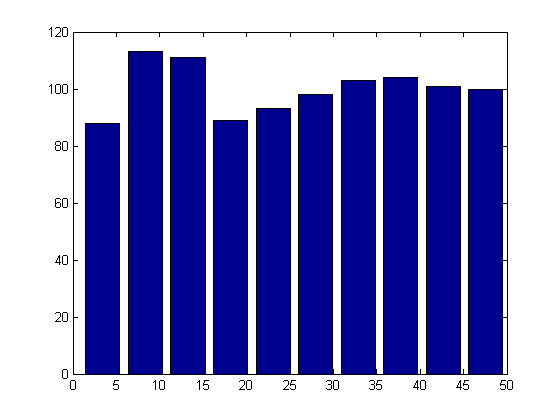
\includegraphics[scale=1]{Figures/1000_agents_color_cluster}
\caption{Color Clusters}
\label{fig:color_clusters}
\end{figure}


Like for any project with a large number of agents, a clear and easy to understand presentation of the simulation was imperative.
Initially the author went with 2-D histograms depicting the membership values of each color group, which presented nicely how the members moved around as the height of the  bars representing the number of members in a group could be easily seen to rise or fall, and the speed of this descent or ascent would tell about the rat of success or failure for a particular color. An example could be seen in figure~\ref{fig:color_clusters}.

\begin{figure}
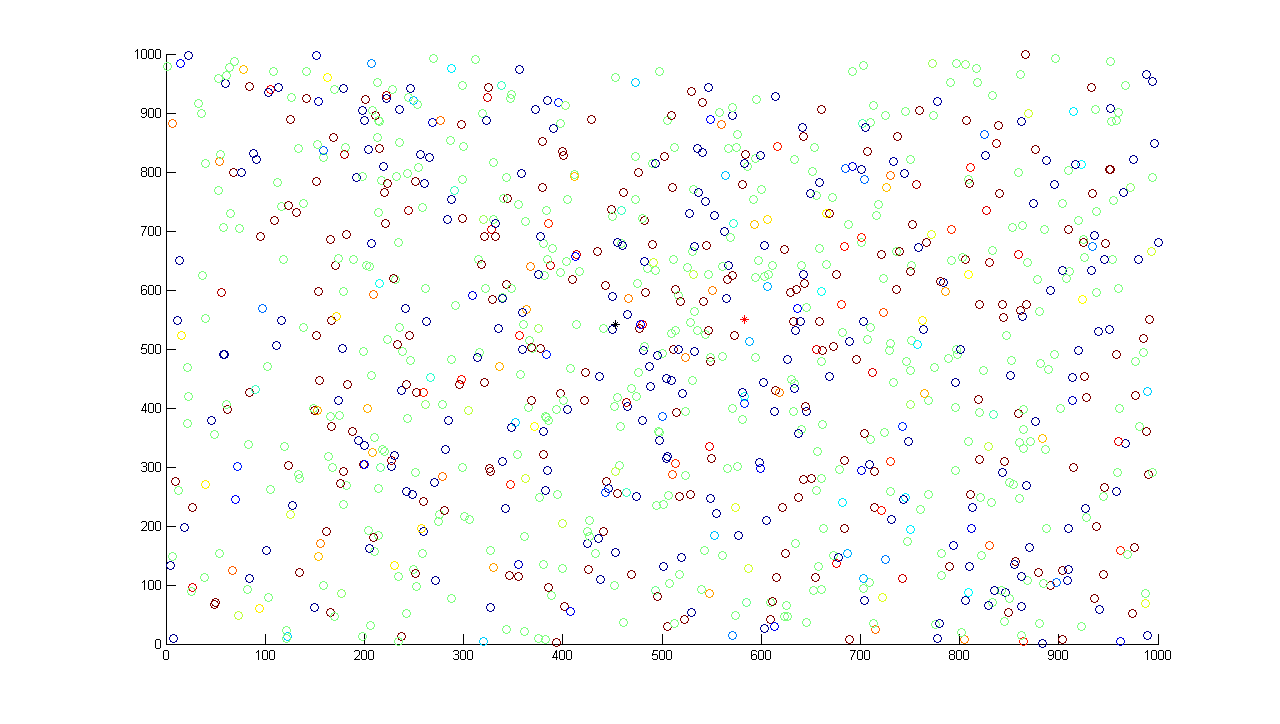
\includegraphics[scale=0.5]{Figures/spatial}
\caption{3-D Spatial Cluster}
\label{fig:spatial_clusters}
\end{figure}



However, with the progress of the model this model became obsolete as it was unable to represent the aspect of ``Cost" to a company. 
To address this necessity, the author decided to switch to a 3-Dimensional presentation, with X- and Y- axes representing generic movement for agents, and the movement or effort as well as incurred cost for the companies, ad the color, being the 3-rd dimension of the presentation, depicting the value of the attribute. The speed of movement here serves the purpose as the speed of rise/fall in the previous model. An example of this is figure ~\ref{fig:spatial_clusters}.

While the X-Y movement in this model, for the agents, is a correlation, the changing colors as they move represent the agents leaning towards or away from a particular company.

%-----------------------------------
%	SUBSECTION 5
%-----------------------------------
\subsection{Company Policies}
\label{sec:policies}
Different companies may have different policies towards customer involvement. 

The customer involvement continuum followed by the author is influenced by the works of Bodil Sanden~\cite{bodil} and follow the categorization by Ives \& Olson ~\cite{1984}.
These categories are :

\begin{enumerate}

\item[1] No involvement. Users are unwilling or not invited to participate.
\item[2] Symbolic involvement. User input is requested but ignored. 
\item[3] Involvement by advice. User advice is solicited through interviews
or questionnaires.
\item[4]  Involvement by weak control. Users have sign-off responsibility at
each stage of the system development process. 
\item[5] Involvement by doing. A user as design team member or as the
official liaison with the information system’s development group. 
\item[6] Involvement by strong control. Users may pay directly for new
development output from their own budget or the users’ overall
organizational performance evaluation is dependent on the
outcome of the development effort. 
\end{enumerate}

Out of these, this thesis focuses on categories 2 and 5.
These two specific categories were chosen because they represent most dissimilar choices while still avoiding the extreme conditions, which allowed the model to simulate the more probable scenarios.

%-----------------------------------
%	SUBSECTION 6
%-----------------------------------
\subsection{Simulation Approach}

The simulation in this thesis focuses on companies attracting agents towards their cause, and the cost incurred in terms of efforts on the part of the company.
The model witnesses three types of potential interactions : 
\begin{enumerate}
\item[1] Company to Agent interaction 

These interactions are predefined, in a sense that a certain number of agents already seeded to believe in a company at the beginning of the simulation. This is explained further in Chapter ~\ref{Chapter3}.

\item[2] Agent to Agent interactions

These interactions are the means by which one agent may influences another to lean towards a company. In this model, the agents belonging to either of the companies in question are referred to as  \emph{influencing agents}, and the others are referred to as \emph{influenced agents}. This also mimics real life as the connections betweens agents are directional.

\item[3] Agent to Company interactions

Whenever an agent is influenced, during the simulation, this also causes the company to make some effort, the amount of which depends on its policies. These interactions are what cause the cost to the company.


\end{enumerate}

The outcome of these interactions are measured by the following two values

\begin{enumerate}
\item[a] Gain

This refers to a success for a company in influencing an agent to lean towards itself.

\item[b] Cost

This refers to the cost incurred to the company and is a fucntion of the effort taken by the company. It depends on the policy being followed by the company.
\end{enumerate}
	





%-----------------------------------
%	SECTION 2
%-----------------------------------

\section{Tools}
As a requirement from the University, Matlab was chosen as the programming language, and no special toolboxes were used.
The curve fitting app was used occasionally to check the output of the simulation.

The formulas, and variants thereof, used by the author were sometimes first tested as a prototype in Python with NetworkX and Mathematica for mathematical validation. However, any of those implementations do not directly contribute to the result.
 
	% Chapter Template

\chapter{Methodology} % Main chapter title

\label{Chapter3} % Change X to a consecutive number; for referencing this chapter elsewhere, use \ref{ChapterX}

\lhead{Chapter 3. \emph{Methodology}} % Change X to a consecutive number; this is for the header on each page - perhaps a shortened title

On an abstract level, the model consists of an environment comprising of numerous agents, and a few companies. This thesis specifically focuses on the various strategies used by the companies to attract the agents, and try to measure its efficiency in terms of the related costs and benefits. Based on these measurements, a company could determine the optimal strategy to maximize its efficiency for the targeted section or sub-subsection of agents.

%----------------------------------------------------------------------------------------
%	SECTION 1
%----------------------------------------------------------------------------------------

\section{The Companies}

The companies only exist in a superficial form in the model. In this model, each company plays the role by providing a central point for the agents to cluster about, and the movement of this point itself denotes effort made by the company, which in turn incurs a cost to the company.

The author decided to keep this model limited to two companies competing for the same spot, i.e., any agent cannot totally belong to both companies at the same time. 


%-----------------------------------
%	SECTION 2
%-----------------------------------
\section{The Agents}

The agents in this model are simpler constructs, each  having a ``color" attribute, and this attribute changes as the agents tend to believe in either of the companies.

Structurally, each agent has following attributes :

\begin{enumerate}
\item ID
\item x-position coordinate
\item y-position coordinate
\item Color value
\item Influence value
\end{enumerate}

%-----------------------------------
%	SECTION 3
%-----------------------------------

\section{Connections}
The connections between the agents form in such a manner that the model satisfies the requirements of free-scaling. 
Following in the footsteps of the giants, the implementation is based on the B-A algortithm [REF] .

\subsection{The World}
The model is first built based on 2 fixed parameters, and then the simulation runs on it.
The author starts building the model for a fixed umber of total agents, and predefined average connectivity in the environment.
The initialization of the model begins with the creation of a small, fully connected network, and then, with time, new agents are added to this network, and these agents form the connections following the rules of PA.
The exact method for forming this connection was modified by the author, so as to further trick the environment and simulate scenarios of chances of connection being formed, but only a fraction of those connections actually being formed. This was achieved by employing a `weight' modifier on the probability of an agent to form a connection. This weight, in turn, is defined for every possible pair of agents, and is based on the difference in the value of a special attribute ``likemindedness", defined for each agent in an uniform, pseudo-random manner.
This attribute is not considered an essential attribute because it may or may not be used, in various simulations. However, as an effect of using this modifier, the number of connections for an agent comes down considerably, while the nature of the connections still remain same, and the network remains scale free.


\subsection{The Simulation} 
 
The simulation begins with allocating ``influence" value to each agent, as a function of the number of connection it makes. This makes sure that the most-connected agents get a chance to be more influential. 
After this, values are uniformly assigned to all agents for the ``color" attribute, and then they are seeded to belong to different companies. 20 \% was the value chosen by the author for initial amount of seeding, for the following combination of reasons:

\begin{enumerate}
\item It allows for equal amount of seeding in both companies.
\item It allows for double amount of seeding in a neutral company.
\item After above mentioned allocations, it leaves equal amount of distribution randomly, to simulate chance.
\end{enumerate}

The above rules give us the formula

$company_1 + company_2 + company_{neutral} + company_{random} = 100$

which translates as

$x + x + 2x + x = 100 \%$

and results in 

$x = 20 \%$ .

Then, we begin running the simulation, where in each time step, an edge is selected randomly, and an exchange could happen if the FromNode of this edge belongs to one of the two companies. Here, and from now onwards, ``belonging to company" refers to the value of the ``color" attribute for the agent.
After this, the influence value of the FromNode is subjected to a randomly selected threshold, and upon satisfaction, the actual communication occurs.
The selection of the edge depicts existence of a connection, while satisfaction of the threshold depicts the actual communication. This constraint was included to make the simulation model even closer to real-life.

For every successful communication, the agents shift their ``color" attribute a fraction towards the influencing company. This shift also translates to their x-y coordinate, which is shown in the presentation. The important aspect here is that these changes in color and x-y coordinates, while not always causally related, are always correlated. 

For the companies, however, it has different significance. Whenever an agent has moved closer, the companies also make an effort and move some fraction towards the agents. The amount of distance moved by the company represents the effort it makes, and is determined by the company policies. These movements also incurs the cost to the company, and a combined function of the gain and this cost determines the effectiveness of the policy.




%----------------------------------------------------------------------------------------
%	SECTION 4
%----------------------------------------------------------------------------------------

\section{Algorithms}

\begin{algorithm}
\caption{Create Scale-Free Network}
\label{ag1}
\begin{algorithmic}
\STATE N : Input, total number of agents
\STATE D : Input, average number of connections
\IF {$D < N+1$}
	\STATE Form a \emph{fully connected} network with D+1 agents
\ENDIF 
\STATE implement $CG$
\STATE $i \gets D+1$
\WHILE{$i < N$} 
	\STATE $Agent_i \gets newAgent$
	\STATE assign $likemindedness$ [FORM-REF]
	\STATE implement $PA$
	\STATE $k \gets 0$
	\WHILE{$k \leq \frac{D}{2}$}
		\STATE calculate $probability_{basic}$ [FORM-REF]
		\STATE compute $weight$ [FORM-REF]
		\STATE $probability_{attachment} \gets  probability_{basic} + weight$ 
		\STATE $Agent_i$ forms $connection_k$ , based on $probability_{attachment}$
	\ENDWHILE	
\ENDWHILE
\end{algorithmic}
\end{algorithm}

\clearpage

\begin{algorithm}
\caption{Simulation}
\label{alg2}
\begin{algorithmic}
\STATE assign $Company$ centres
\STATE calculate $influence$ [FORM-REF]
\STATE assign \emph{color} to all agents
\STATE seed $20\% $ agents to $color1$
\STATE seed $20\%$ agents to $color50$
\STATE seed $40\%$ agents to $color25$
\STATE seed $2 \emph{most influential}$ agents to different companies
\STATE $J$ : number of iterations
\STATE $i \gets 0$
\WHILE{$i \leq J$}
	\STATE select $edge_i$
	\IF{ $FromNode_{color}$ = $\emph{color1}$ OR $\emph{color50}$ }
		\STATE select $threshold$
		\IF{ $ FromNode_{influence} \geq threshold $ }
			\STATE $ToNode_{color} \gets ToNode_{color} + \emph{shift}$
			\STATE $ToNode_{x-coordinate} \gets ToNode_{x-coordinate} + \emph{shift}$
			\STATE $ToNode_{y-coordinate} \gets ToNode_{y-coordinate} + \emph{shift}$
			\STATE $Company_{x-coordinate} \gets Company_{x-coordinate} + \emph{shift}$
			\STATE $Company_{y-coordinate} \gets Company_{y-coordinate} + \emph{shift}$
		\ENDIF
	\ENDIF
\ENDWHILE
\end{algorithmic}
\end{algorithm}

\clearpage

\section{Definitions}
\begin{enumerate}
\item \emph{Fully Connected}

It follows the standard definition that each node is connected to every other node. The initial network is formed in a manner such that it is fully connected and satisfies the average number of total connections.

\item \emph{Likemindedness}

It is a special attribute of the agents, that is used in this model to modify the probability of formation of a new connection between two agents. It simulates the real life phenomenon that people with similar interests may be more likely to form a connection. This is also helpful in showing the aspect tht some people may be introverts or extroverts. However, that aspect is not simulated in detail in this model [REF].

\item \emph{Weight}

The weight is the difference in likemindedness of two agents. It is calculated as 

$weight_{j,k} = abs( likemindedness{j} - likemindedness{k} )$

\item \emph{Company Centre}

The company is not implemented as a structural entity, rather, the company centre is used to keep track of the attitude of the agents towards the company, and also to track the effort and cost on the part of the company.

\item \emph{Influence}

This attribute determines the chances of an agent to influence another agent. As in real life, we allow more connected agents a chance to be more influential, but ultimately, there is no deterministic end to the model, and whether or not an actual comunication takes place and an agent gets influenced is always determined by a randomly determined threshold.

\item \emph{Shift}

This shift represents a change in the state of the overall system. For an agent, a shift in it's color attribute represents the agent leaning towards a company. This shift is correlated with the same ratio of change in the agent's x-y coordinate, used for visualization purposes.
For a company, the shift only occurs in it's x-y coordinate, which is caused by the x-y shift of the agent, and this change represents two things : 
\subitem[A] The speed and frequency of movement represent the effort taken by the company
\subitem[B] The distance moved represent the cost incurred to the company
\end{enumerate}
% Chapter Template

\chapter{Experimental Results} % Main chapter title

\label{Chapter4} % Change X to a consecutive number; for referencing this chapter elsewhere, use \ref{ChapterX}

\lhead{Chapter 4. \emph{Experimental Results}} % Change X to a consecutive number; this is for the header on each page - perhaps a shortened title

%----------------------------------------------------------------------------------------
%	SECTION 1
%----------------------------------------------------------------------------------------

\section{The Model}

The most common form of representing a scale-free network is by using its degree of connections, where the horizontal axis represents number of connections, and the vertical axis represents the number of agents having that many connections.

\begin{figure}
\centering
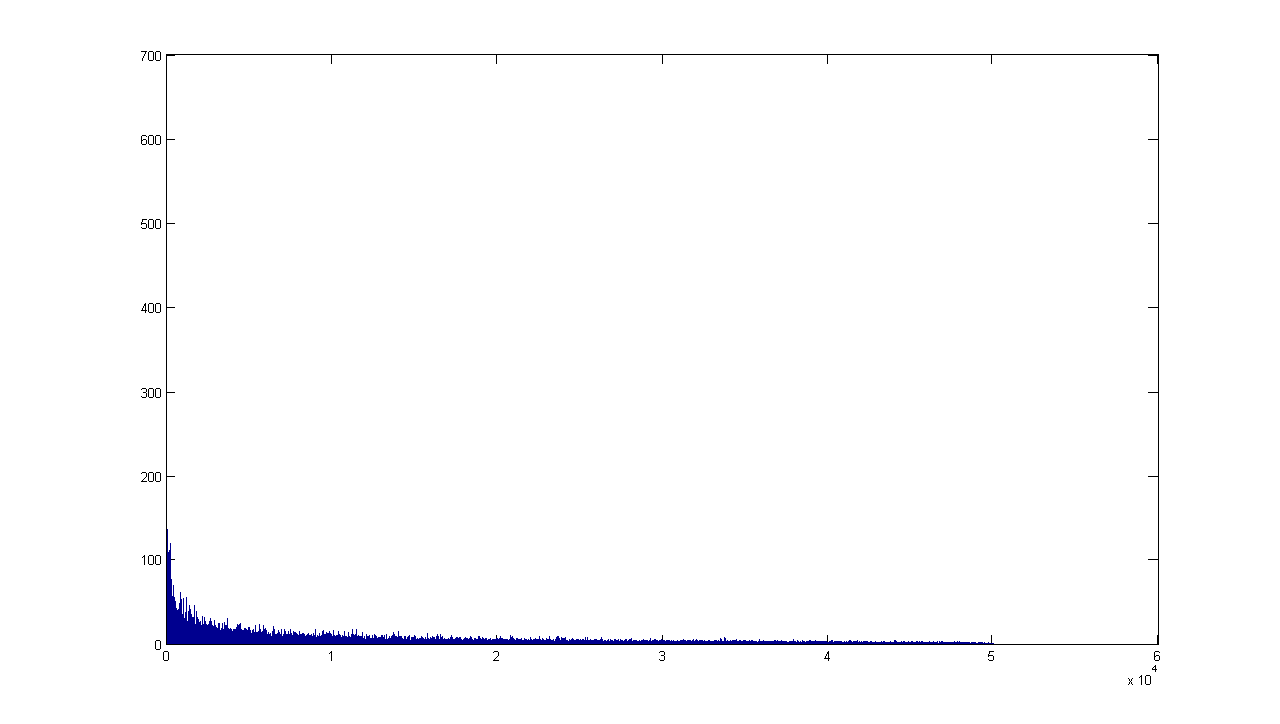
\includegraphics[scale=0.5]{Figures/50000m1_small_world}
\caption[Small World Network with Original Algorithm]{Small world Network, Original BA algorithm}
\label{fig:small_world_original}
\end{figure}

\begin{figure}
\centering
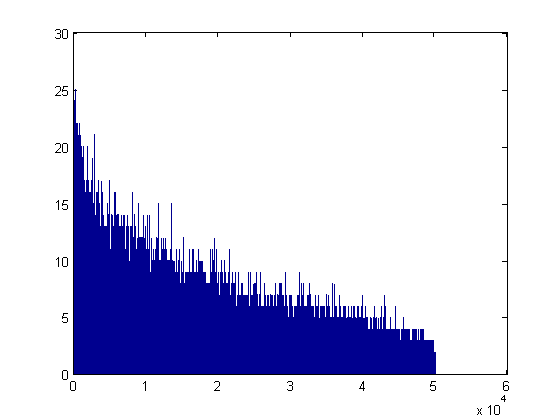
\includegraphics[scale=0.75]{Figures/50000m2_small_world}
\caption[Small World Network with Modified Algorithm]{Small world Network, Modified BA algorithm}
\label{fig:small_world_modified}
\end{figure}

Figures~\ref{fig:small_world_original} and ~\ref{fig:small_world_modified} show the different degrees in the connection in the case of using original BA algorithm and using our modified approach to the algorithm respectively.

It can be observed that using the constraint of `likemindedness' results in a drop in the horizontal axis values, which shows that lesser number of connections are formed.

The basic model was modified a lot with time, from the initial design, as the author learnt more. The development of the model can be explained in two parts.

%-----------------------------------
%	SUBSECTION 1
%-----------------------------------
\subsection{Small-World Networks}
Figures~\ref{fig:small_world_original} and ~\ref{fig:small_world_modified} both show discontinuation in the tail. 

On further inspection, it was found that the networks were displaying characterictics of Small-World networks~\cite{smallWorld}. The difference in what was required and what was achieved is made clear by Cohen \& Havlin~\cite{PhysRevLett.90.058701}.

This led to modifications in the design and the design explained in Chapter~\ref{Chapter3} was achieved.

%-----------------------------------
%	SUBSECTION 2
%-----------------------------------

\subsection{Scale-free Networks}

An example in comparison of both models, i.e., following original BA algorithm and the modified approach, can be seen in Figure~\ref{fig:scaleFree_comp}, where green color represents the original algorithm and blue represents the modified approach.

\begin{figure}
\centering
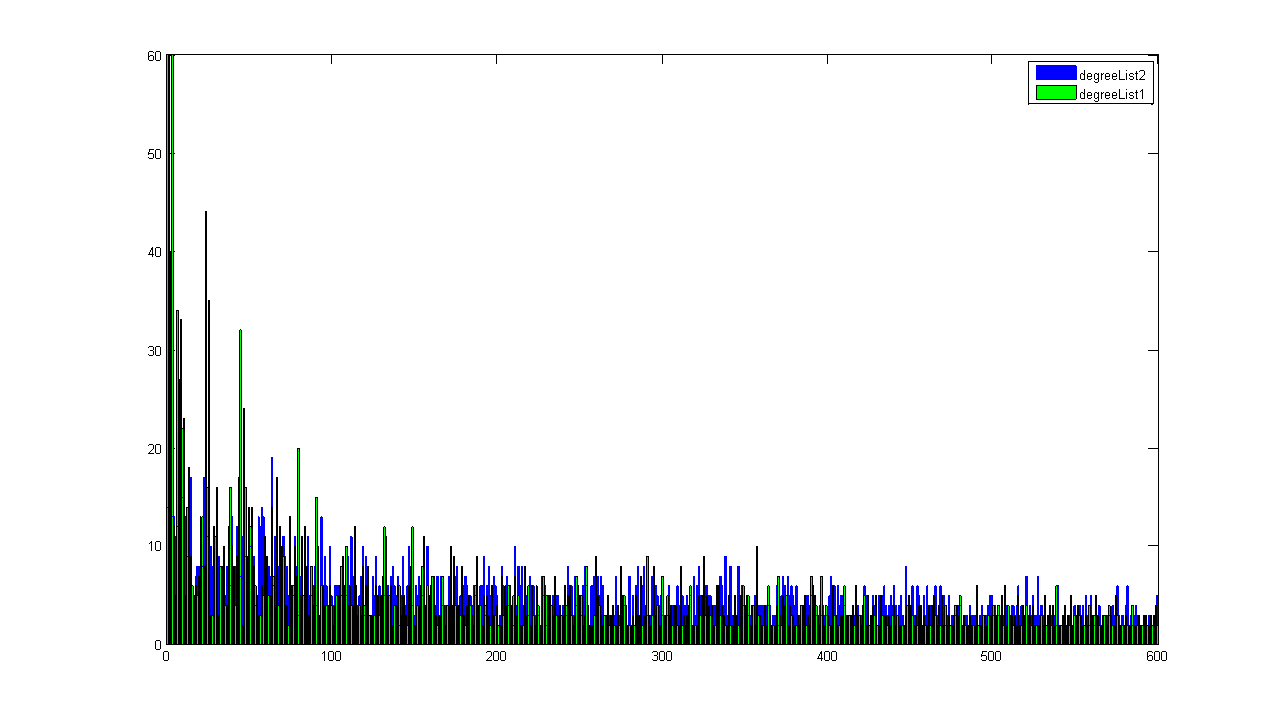
\includegraphics[scale=0.5]{Figures/scaleFree_comparison}
\caption[Comparison of Scale Free Networks]{Comparison of Scale Free Networks generated by the different algorithms for 1000 agents}
\label{fig:scaleFree_comp}
\end{figure}

These outputs were further tested for fit, using MATLAB's curve fitting toolbox, against a power-law curve, and the results are shown in figure~\ref{fig:power1} and ~\ref{fig:power2}.

\begin{figure}
\begin{center}$
\begin{array}{cc}
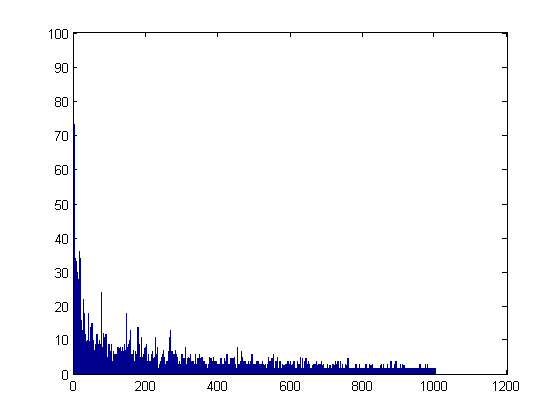
\includegraphics[scale=0.5]{Figures/1000m1} \\
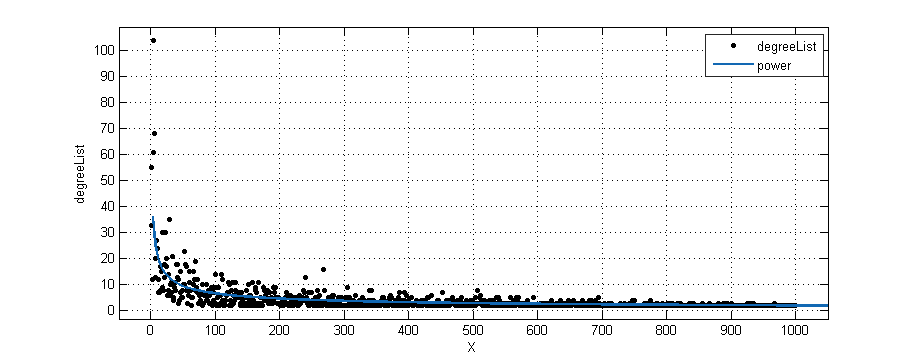
\includegraphics[scale=0.5]{Figures/1000m1_powerFit} 
\end{array}$
\end{center}
\caption[Power Law Fit for Original Algorithm]{Scale-Free network using BA algorithm and corresponding power law fit}
\label{fig:power1}
\end{figure}

\begin{figure}
\begin{center}$
\begin{array}{cc}
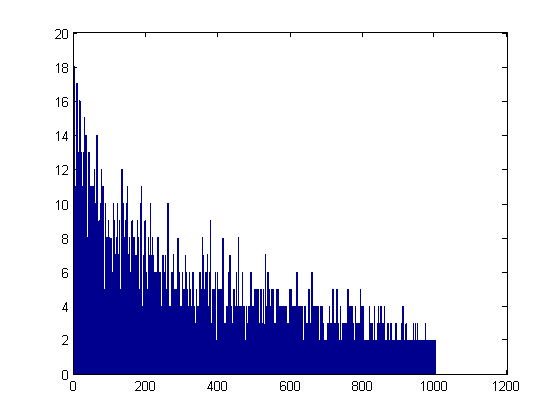
\includegraphics[scale=0.5]{Figures/1000m2} \\
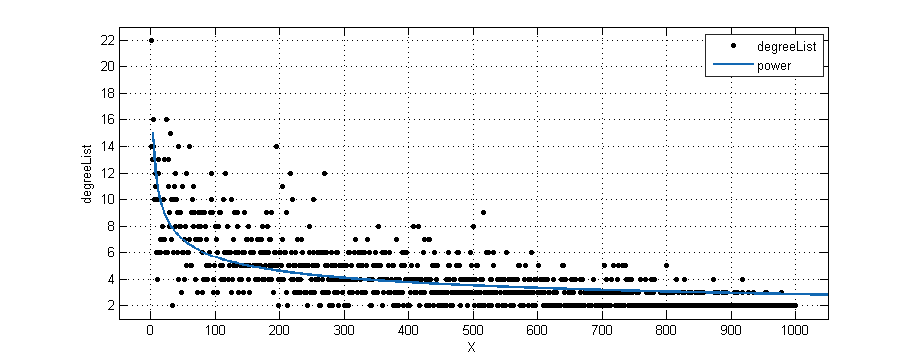
\includegraphics[scale=0.5]{Figures/1000m2_powerFit} 
\end{array}$
\end{center}
\caption[Power Law Fit for Modified Algorithm]{Scale-Free network using modified BA algorithm and corresponding power law fit}
\label{fig:power2}
\end{figure}


%----------------------------------------------------------------------------------------
%	SECTION 2
%----------------------------------------------------------------------------------------

\section{The Simulation}

The simulations resulted in three different types of outputs. They were all run for cases where on an average, every agent makes 3 connections. The different types of outputs are as follows:

\begin{enumerate}
\item[1] Color Histograms
\item[2] Spatial Clusters
\item[3] Cost-Gain Functions
\end{enumerate}

For the specific purposes of this thesis, spefically for analysis part, a particular set of `Gain' and `Cost' values, in accordance with the policies followed by the companies, were used. Keeping the gain for each influence fixed at `One' unit, and allowing the agents to move 0.2 percent of the distance at a single step, the costs are varied as per table~\ref{table:cost}.

The costs are also equal to the effort, i.e., the amount of fraction of distance travelled by the company towards the agent.

\begin{table}
\begin{center}
\begin{tabular}{|l||c|r|}
\hline
caseId & cost1 & cost2 \\ \hline 
Base1 & 0.001 & 0.001 \\ 
Base2 & 0.002 & 0.002 \\
Base3 & 0.01 & 0.01 \\
Base4 & 0.02 & 0.02 \\
Diff1 & 0.001 & 0.002 \\
Diff2 & 0.001 & 0.01 \\
Diff3 & 0.001 & 0.02 \\
Diff4 & 0.002 & 0.01 \\
Diff5 & 0.002 & 0.02 \\
Diff6 & 0.01 & 0.02 \\
\hline
\end{tabular} 
\caption[Cost ]{Costs for various cases for both the companies}
\label{table:cost}
\end{center}
\end{table}

%-----------------------------------
%	SUBSECTION 1
%-----------------------------------
\subsection{Color Histograms}

These histograms give the observer a good view of how the agents tend to lean from one company towards another.

Since the network has a large concentration of agents initially seeded to a neutral color which is equidistant from both company1 and company2, it could be observed that a huge initial spike is in the center, while the two companies in question are at the extreme corners.

The change in the heights of different columns can be seen in fig.~\ref{fig:cluster1}. The horizontal axis represents the color value, and the vertical axis represents the number of agents having that value for the color attribute, or, in other terms, the membership of that company.

Fig.~\ref{fig:cluster2} shows a similar output for 10000 agents. This case shows that although the agents move away from the central, equidistant clusters, they may not always reach all the way to either of the company clusters. This is evident by the change of height of the intermediate columns.

\begin{figure}
\begin{center}$
\begin{array}{cc}
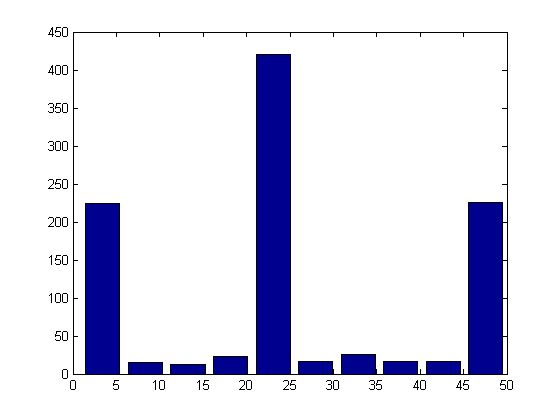
\includegraphics[scale=0.5]{Figures/1000_m2_initial}
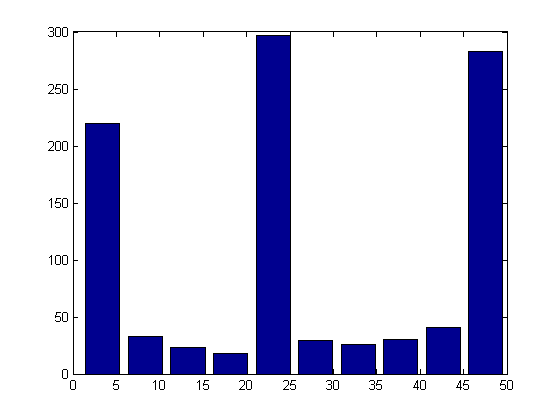
\includegraphics[scale=0.5]{Figures/1000_m2_final} 
\end{array}$
\end{center}
\caption[Color Clusters 1]{Color Clusters for 1000 agents. Initial Cluster on left, and final clusters on right.}
\label{fig:cluster1}
\end{figure}

\begin{figure}
\begin{center}$
\begin{array}{cc}
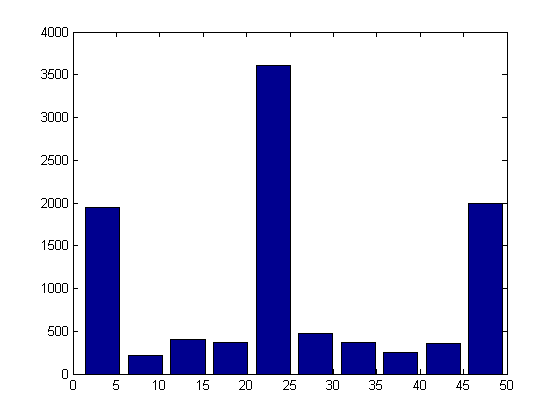
\includegraphics[scale=0.5]{Figures/10000_m2_initial}
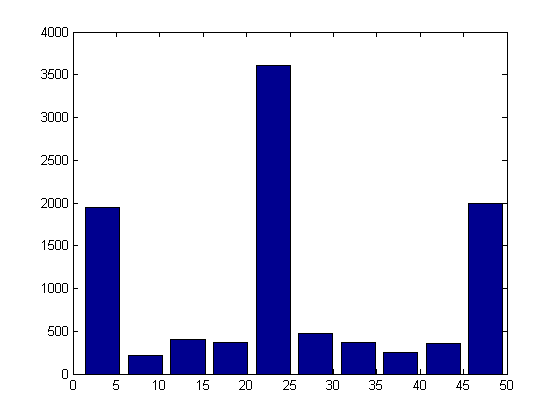
\includegraphics[scale=0.5]{Figures/10000_m2_final} 
\end{array}$
\end{center}
\caption[Color Clusters 2]{Color Clusters for 10000 agents. Initial Cluster on left, and final clusters on right.}
\label{fig:cluster2}
\end{figure}


%-----------------------------------
%	SUBSECTION 2
%-----------------------------------

\subsection{Spatial Cluster}

As mentioned in chapter~\ref{Chapter2}, section~\ref{sec:presentaion}, these outputs were necessary to visualise the cost incurred to the companies.
 
The three dimensions of any element of these plots are its x-y coordinates and its color. The agents are visible as `o' markers, while the companies are shown with `*' markers.

The simulation allows the observer to see the agents change their color as they move towards a specific company. Some screenshots of the simulations can be seen in fig.~\ref{fig:spatial1} and ~\ref{fig:spatial2}.

While fig.~\ref{fig:spatial1} is easier on the human-eye, fig.~\ref{fig:spatial2} is a result of a lot more iterations and is richer in terms of analytics.

\begin{figure}
\begin{center}$
\begin{array}{cc}
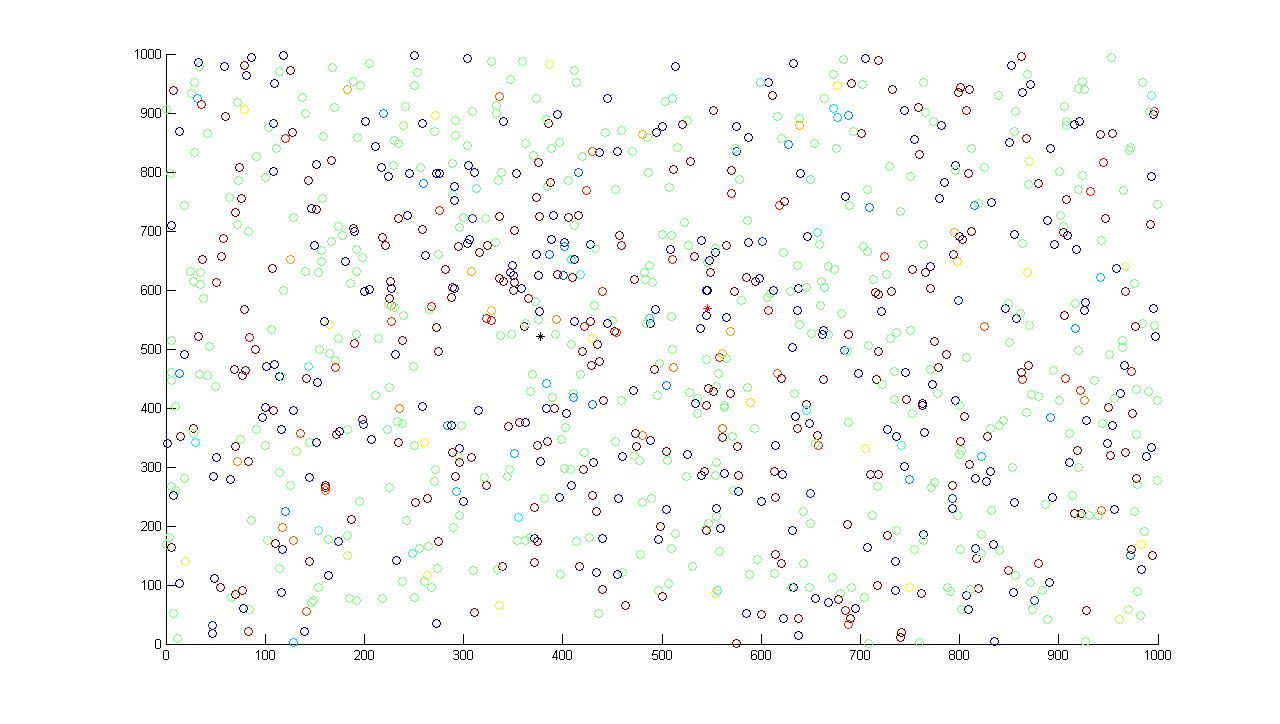
\includegraphics[scale=0.25]{Figures/1000_m2_initial_spatial}
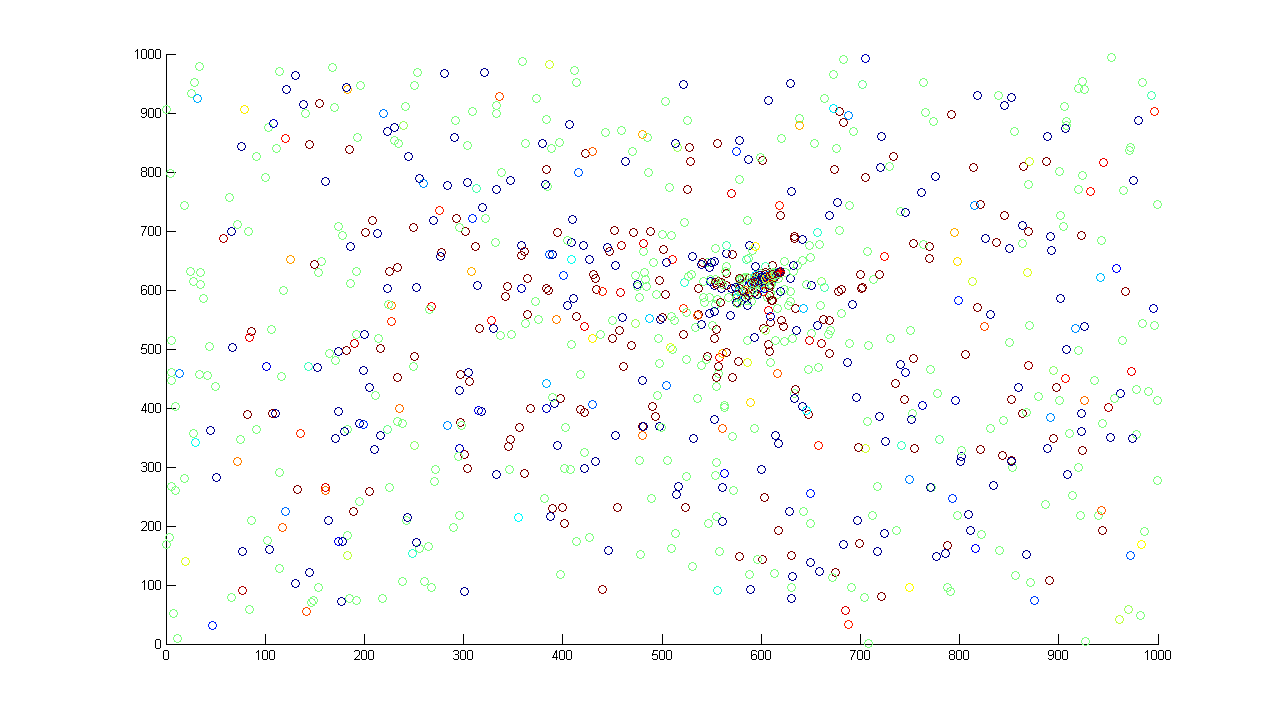
\includegraphics[scale=0.25]{Figures/1000_m2_final_spatial} 
\end{array}$
\end{center}
\caption[Spatial Clusters 1]{Spatial Clusters for 1000 agents. Initial Cluster on left, and final clusters on right.}
\label{fig:spatial1}
\end{figure}


\begin{figure}
\begin{center}$
\begin{array}{cc}
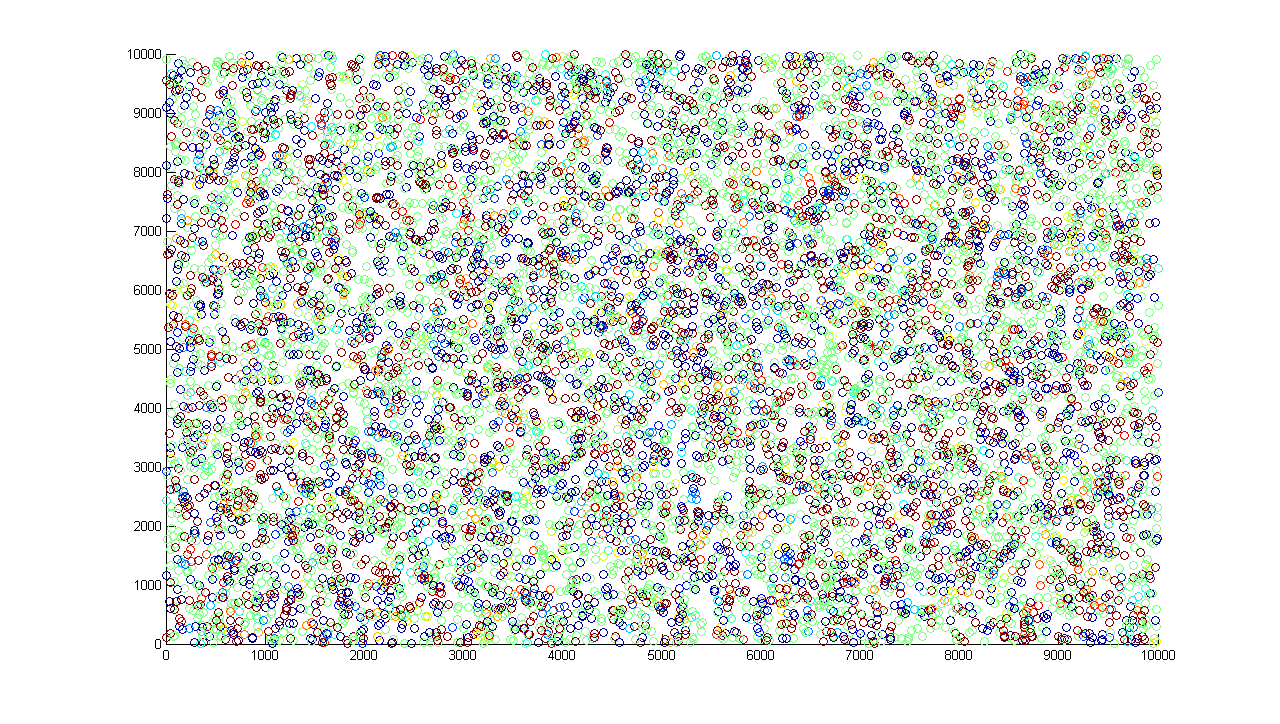
\includegraphics[scale=0.25]{Figures/10000_m2_initial_spatial}
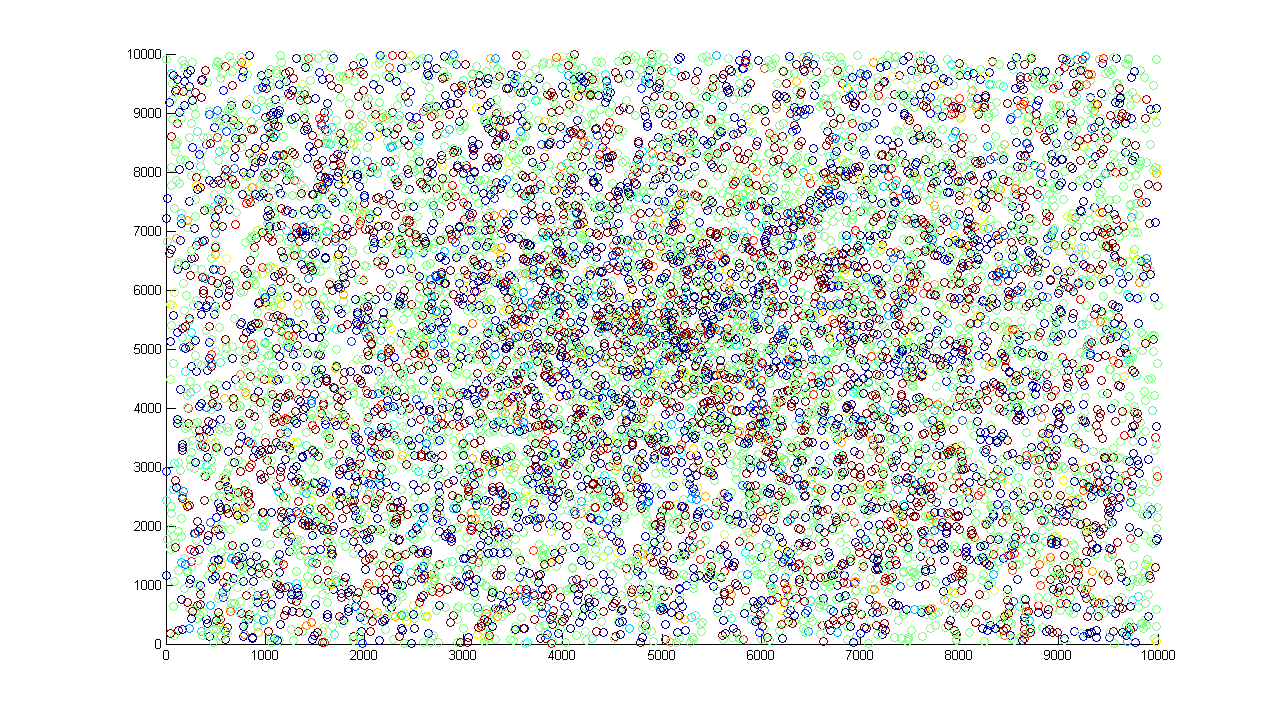
\includegraphics[scale=0.25]{Figures/10000_m2_final_spatial} 
\end{array}$
\end{center}
\caption[Spatial Clusters 2]{Spatial Clusters for 10000 agents. Initial Cluster on left, and final clusters on right.}
\label{fig:spatial2}
\end{figure}


%-----------------------------------
%	SUBSECTION 3
%-----------------------------------

\subsection{Cost-Gain Function}
\label{sec:cost_gain}
The simulation keeps track of the cost and gain for each company according to table~\ref{table:cost}. Company1 follows cost1 while company2 follows cost2, and the caseId tells us about the relation in the policies.

The generic spread and the population count of the companies was monitored, and they tend to show exponential nature of change.

\begin{figure}
\begin{center}$
\begin{array}{cc}
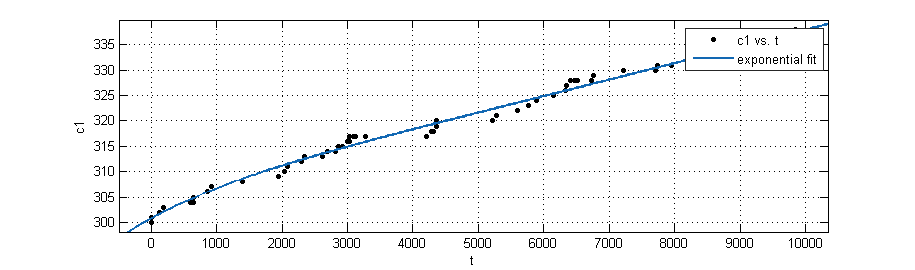
\includegraphics[scale=0.33]{Figures/diffusionTracking_exponentialFit_1000} \\
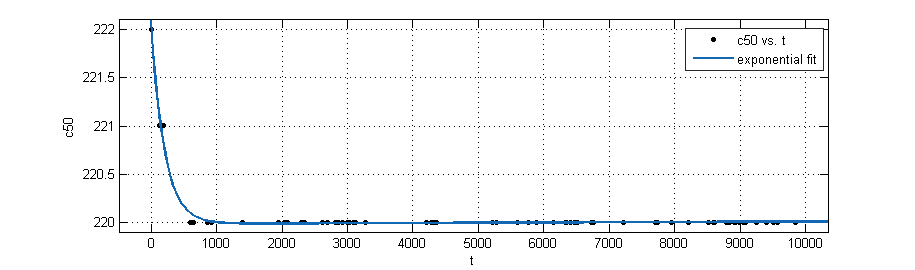
\includegraphics[scale=0.33]{Figures/diffusionTracking_exponentialFit_1000_decrease} 
\end{array}$
\end{center}
\caption[Diffusion 1]{Changes in membership of company for 1000 agents }
\label{fig:diffusion1}
\end{figure}

\begin{figure}
\begin{center}$
\begin{array}{cc}
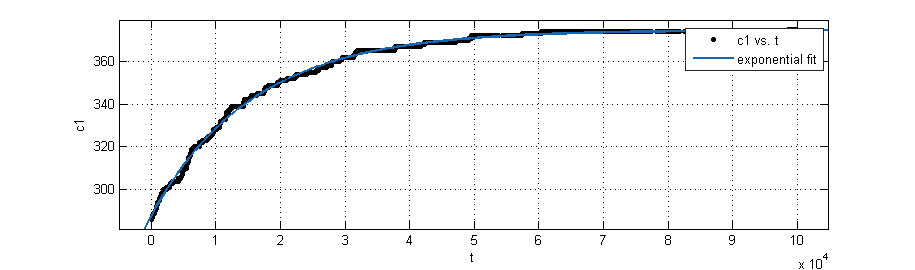
\includegraphics[scale=0.33]{Figures/diffusionTracking_exponentialFit_10000} \\
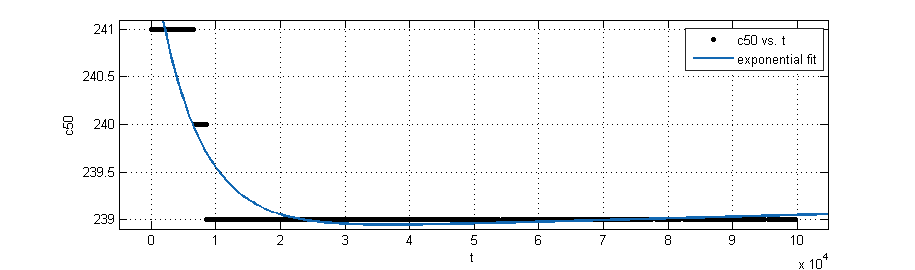
\includegraphics[scale=0.33]{Figures/diffusionTracking_exponentialFit_10000_decrease} 
\end{array}$
\end{center}
\caption[Diffusion 2]{Changes in membership of company for 10000 agents }
\label{fig:diffusion2}
\end{figure} 

Fig.~\ref{fig:diffusion1} and ~\ref{fig:diffusion2} show the increase and decrease of the membership of the companies against exponential fit.

The cases from table~\ref{table:cost} show the functions in the form of equation~\ref{eqn:cost_gain}. These results can be divided into two categories. These are :

\begin{enumerate}
\item[1] \emph{Base} cases

These cases see both companies taking equal cost, and are meant to give the observer an idea about behaviour of both companies under similar policies. The output of these cases can be seen in fig.~\ref{fig:base1},~\ref{fig:base2},~\ref{fig:base3}, and ~\ref{fig:base4}.

\item[2] \emph{Diff} cases
These cases witness the companies following different policies, and allows the observer to analyse the policies. In this approach, cost for Company1 is kept at a constant while the cost for Company2 is increased, and the observed results are recorded. 
The output of these cases can be seen in fig.~\ref{fig:diff1}, ~\ref{fig:diff2}, ~\ref{fig:diff3}, ~\ref{fig:diff4}, ~\ref{fig:diff5}, and ~\ref{fig:diff6}. 

\end{enumerate}

\begin{figure}
\begin{center}$
\begin{array}{ccc}
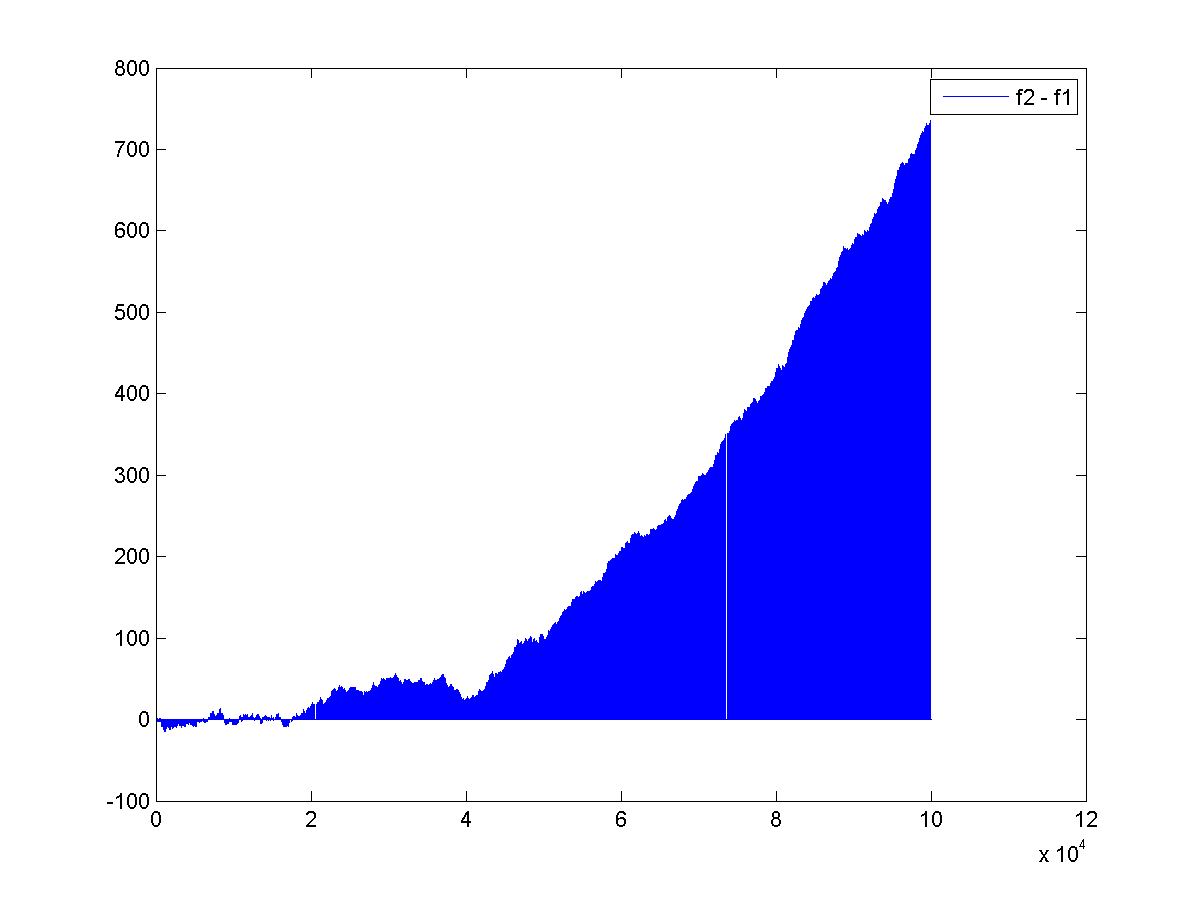
\includegraphics[scale=0.33]{Figures/base1/base1_1} 
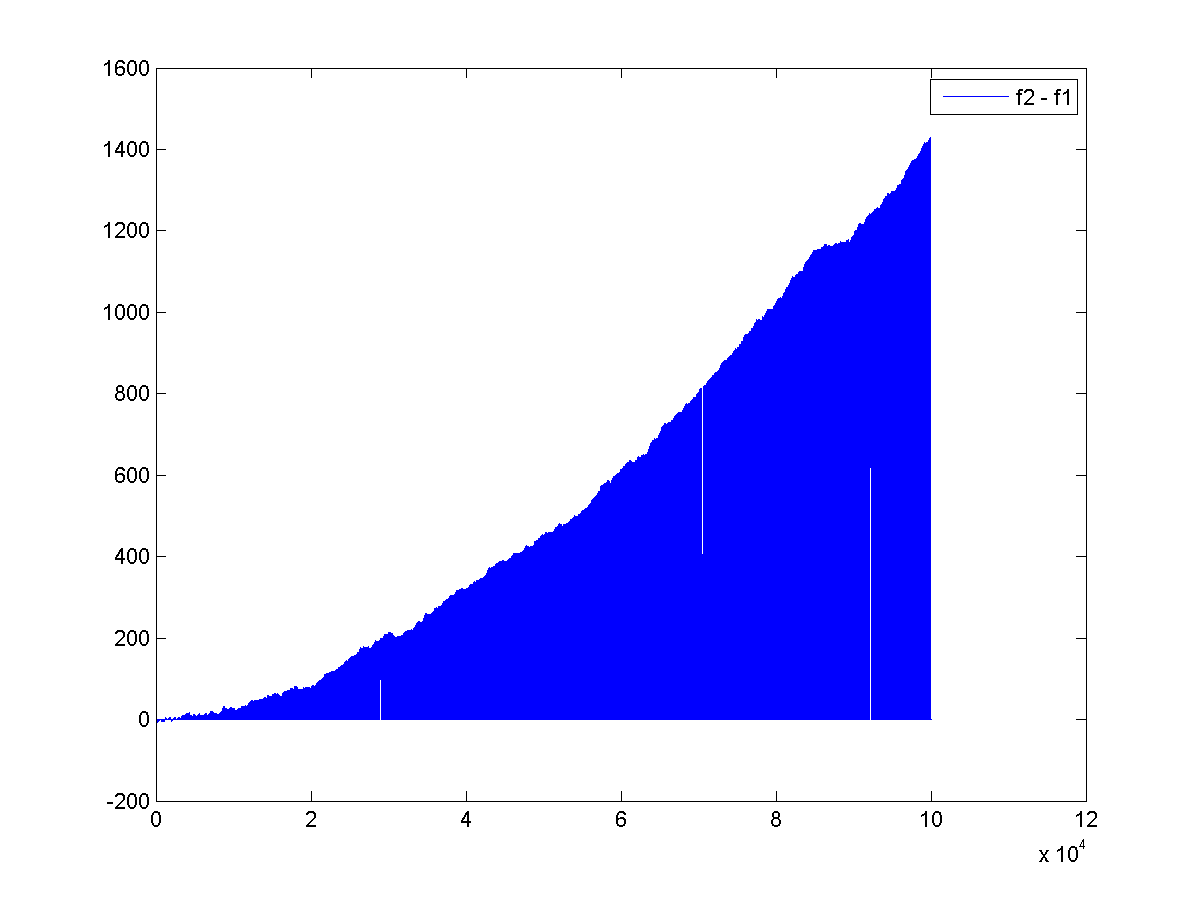
\includegraphics[scale=0.33]{Figures/base1/base1_2} \\
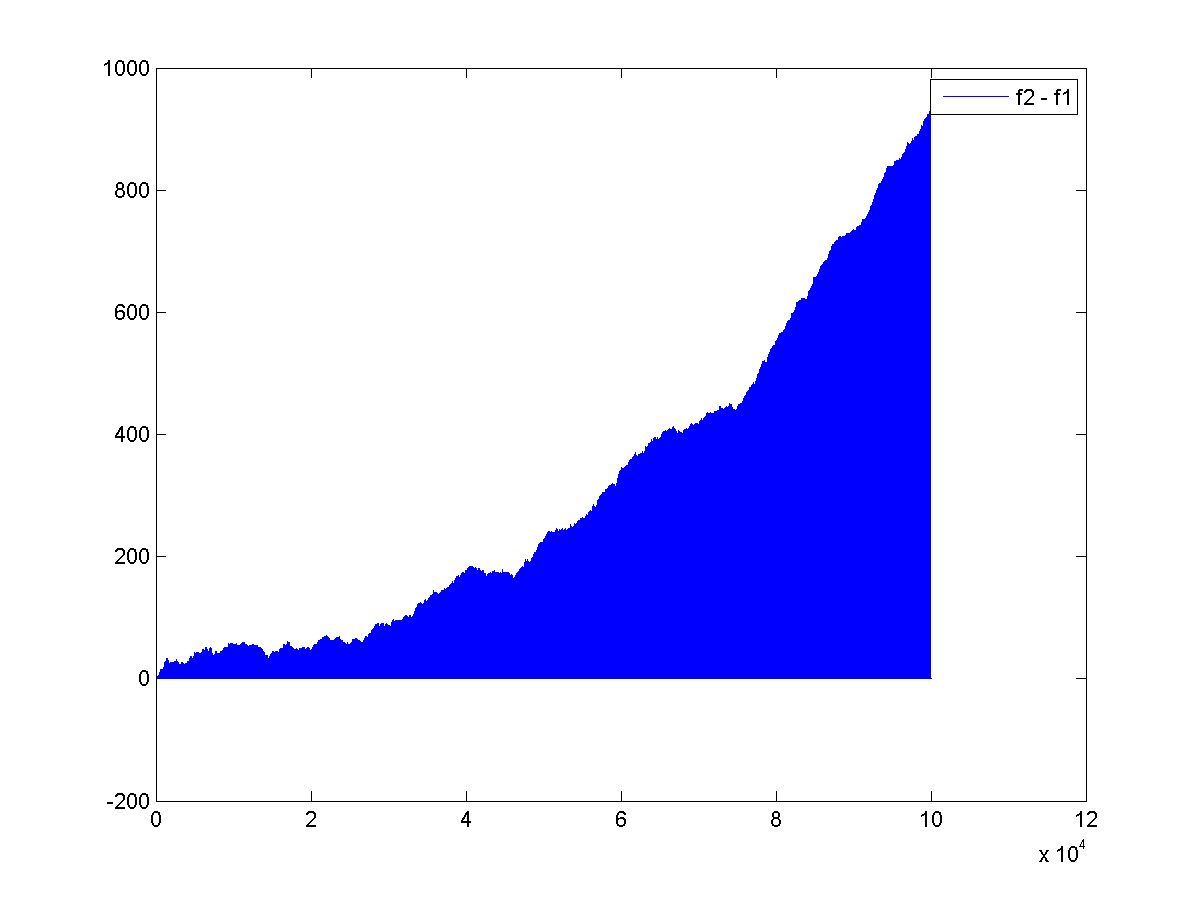
\includegraphics[scale=0.33]{Figures/base1/base1_3}
\end{array}$
\end{center}
\caption[Base case 1]{Results from three simulations for base case 1.}
\label{fig:base1}
\end{figure}

\begin{figure}
\begin{center}$
\begin{array}{ccc}
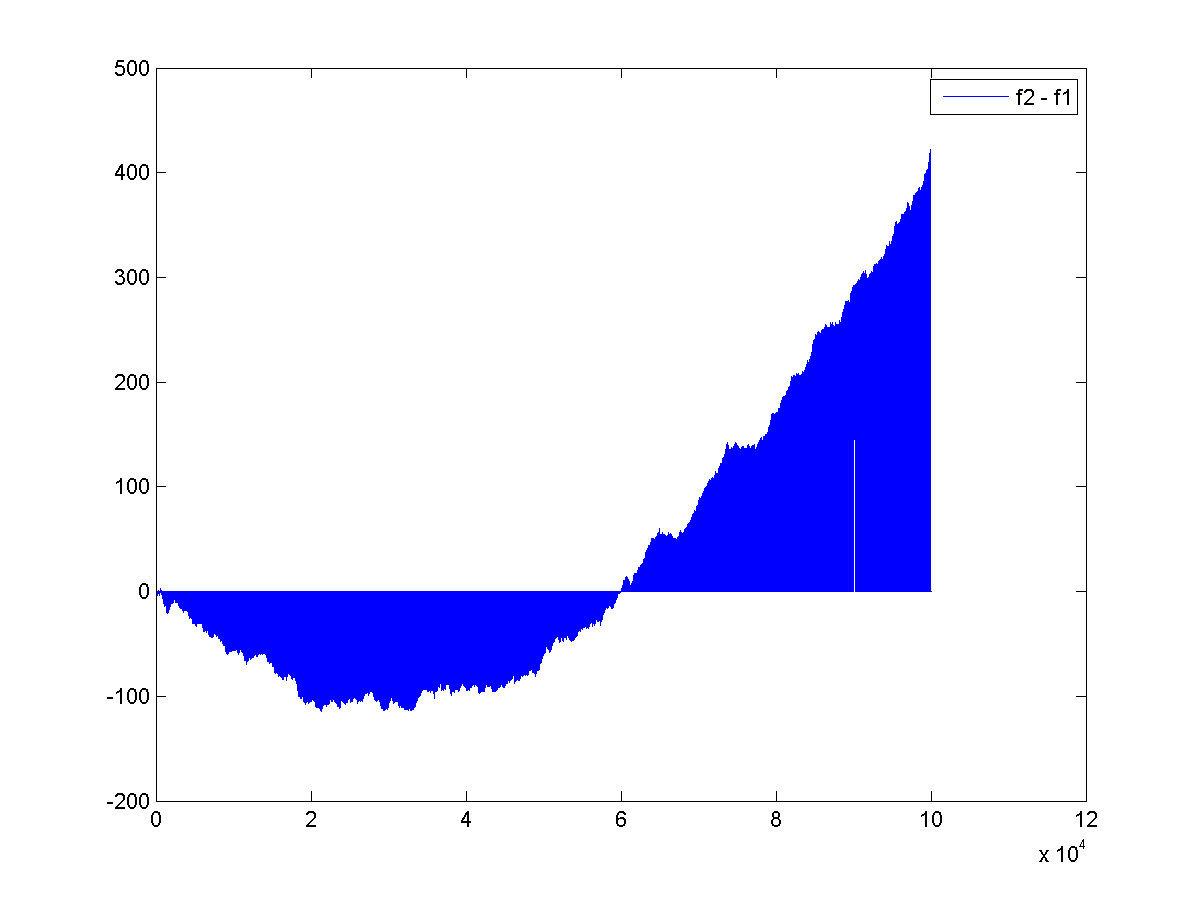
\includegraphics[scale=0.33]{Figures/base1/base2_1} 
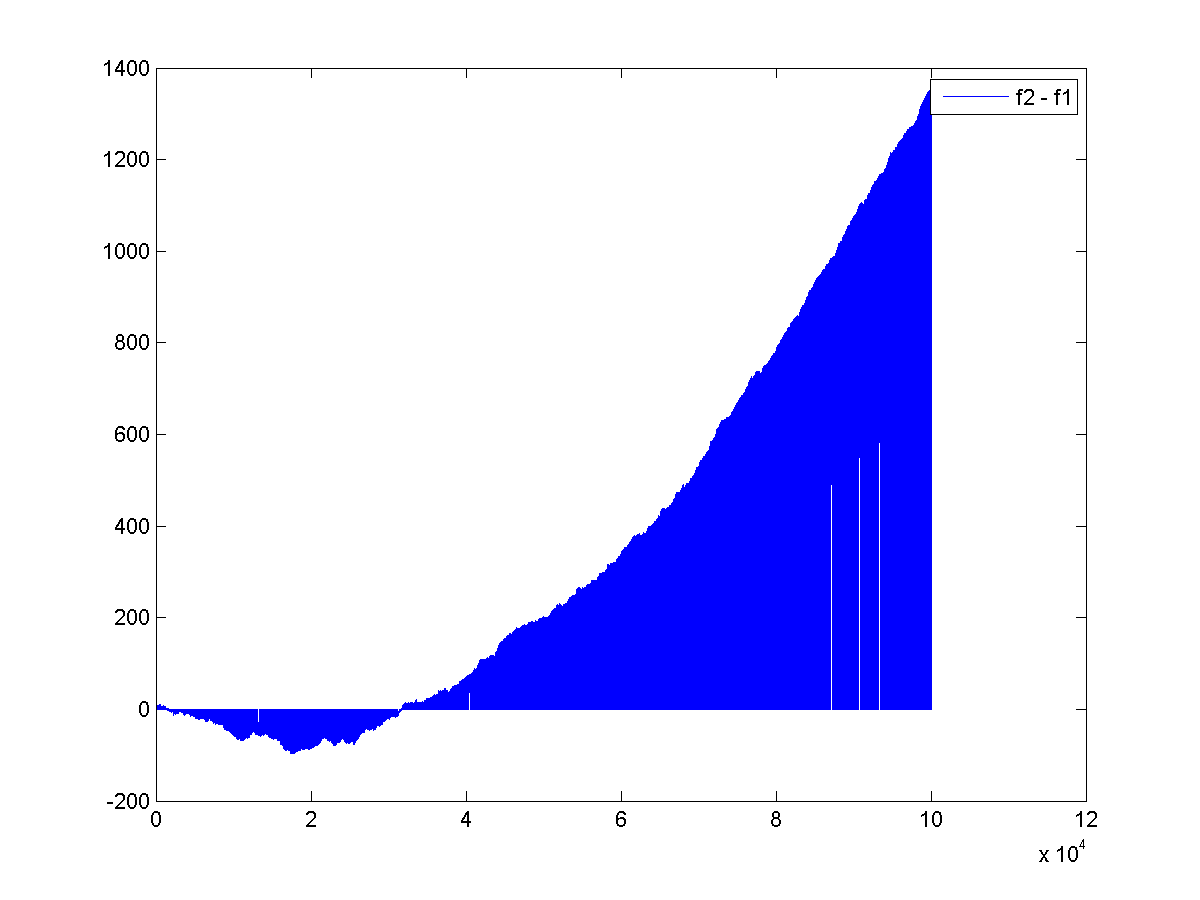
\includegraphics[scale=0.33]{Figures/base1/base2_2} \\
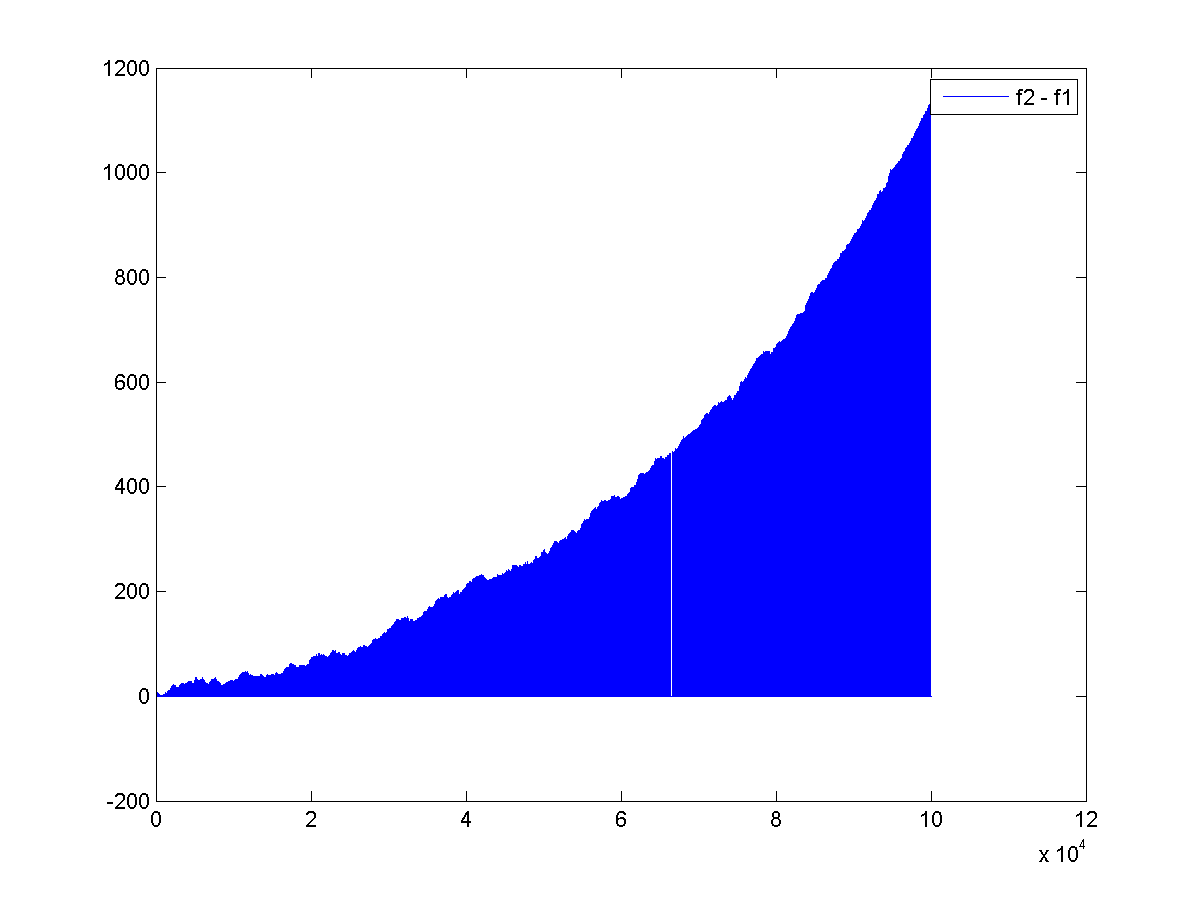
\includegraphics[scale=0.33]{Figures/base1/base2_3}
\end{array}$
\end{center}
\caption[Base case 2]{Results from three simulations for base case 2.}
\label{fig:base2}
\end{figure}

\begin{figure}
\begin{center}$
\begin{array}{ccc}
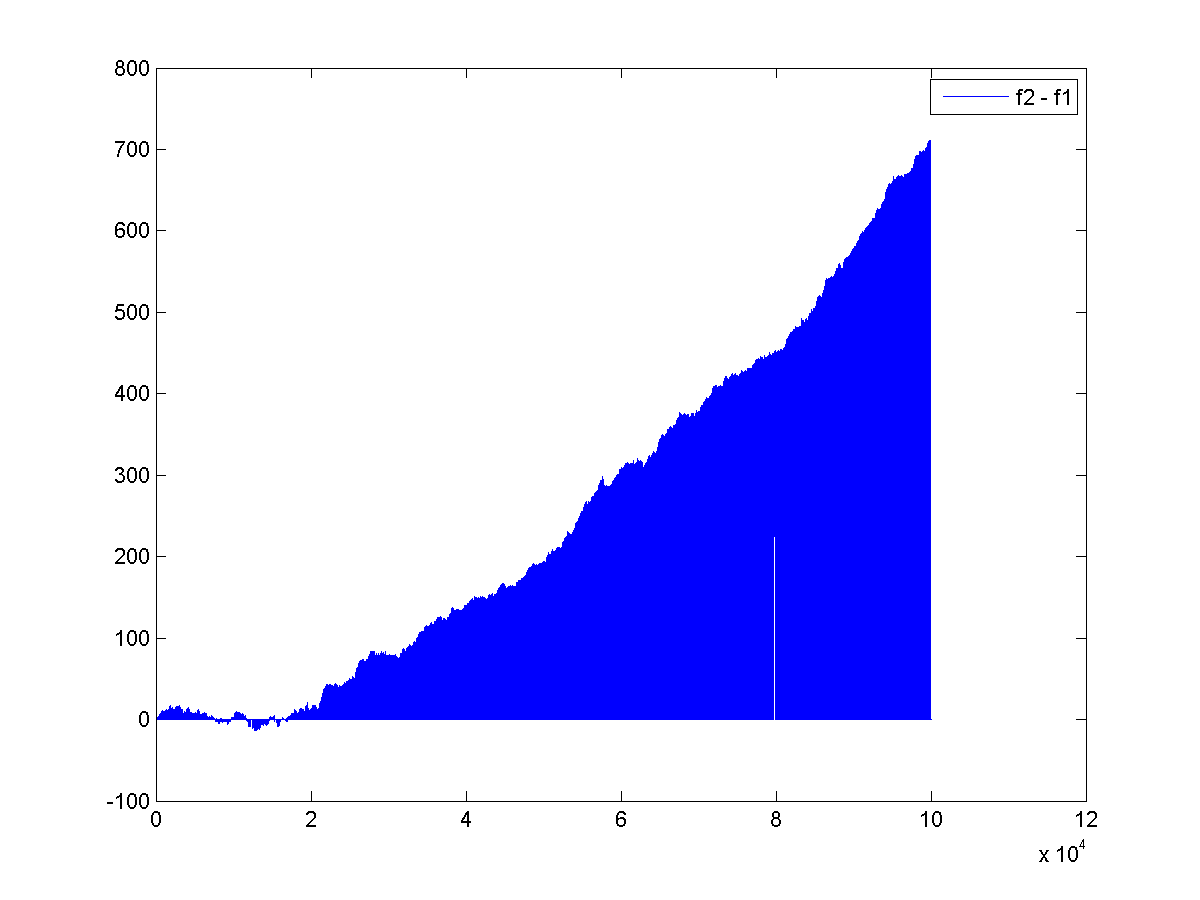
\includegraphics[scale=0.33]{Figures/base1/base3_1} 
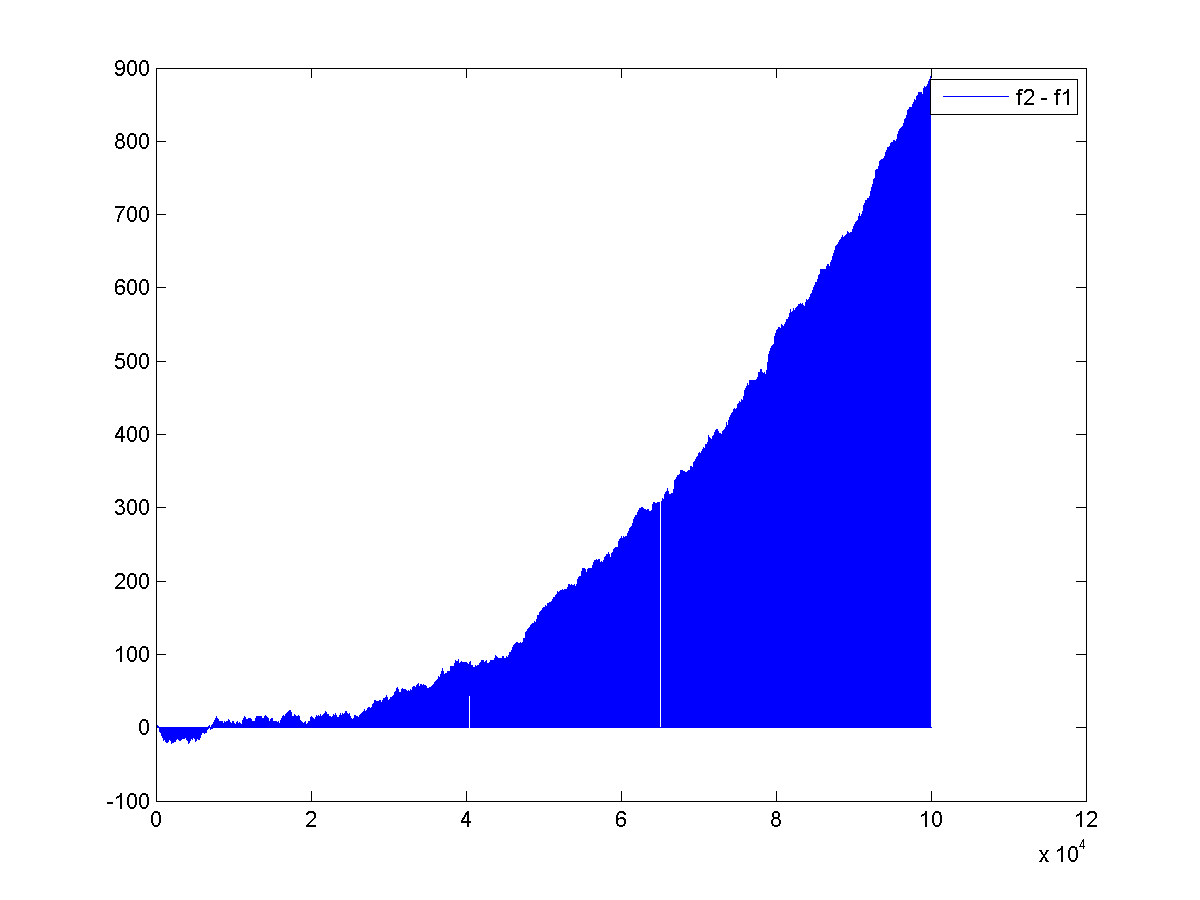
\includegraphics[scale=0.33]{Figures/base1/base3_2} \\
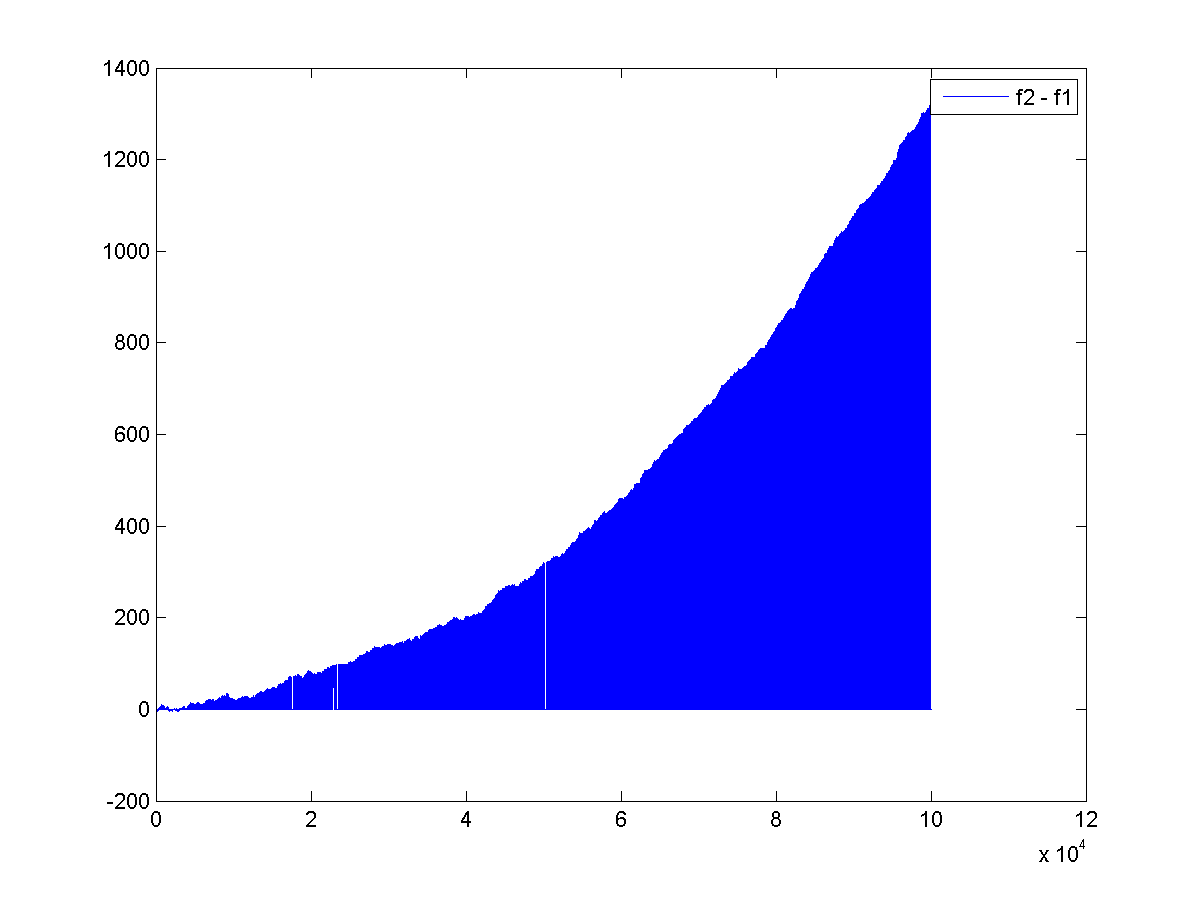
\includegraphics[scale=0.33]{Figures/base1/base3_3}
\end{array}$
\end{center}
\caption[Base case 3]{Results from three simulations for base case 3.}
\label{fig:base3}
\end{figure}

\begin{figure}
\begin{center}$
\begin{array}{ccc}
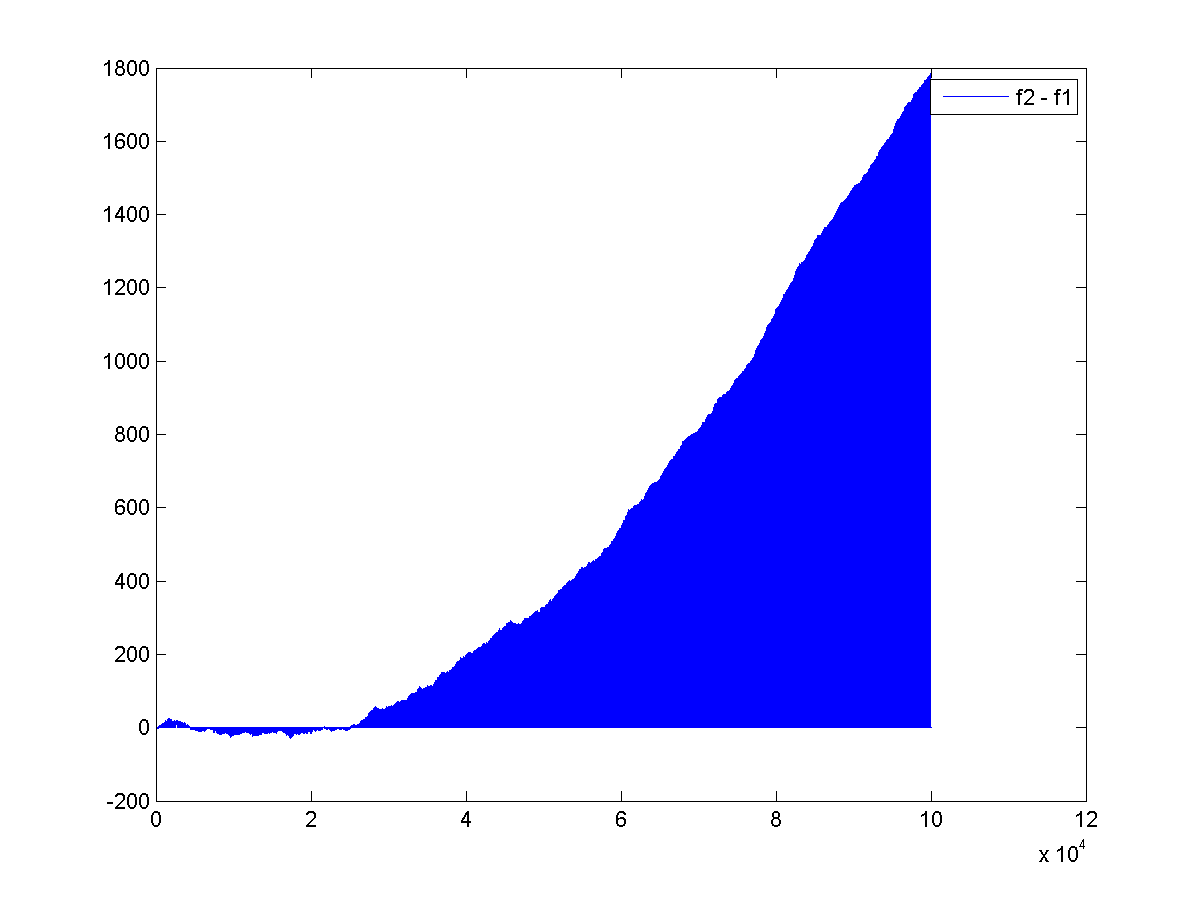
\includegraphics[scale=0.33]{Figures/base1/base4_1} 
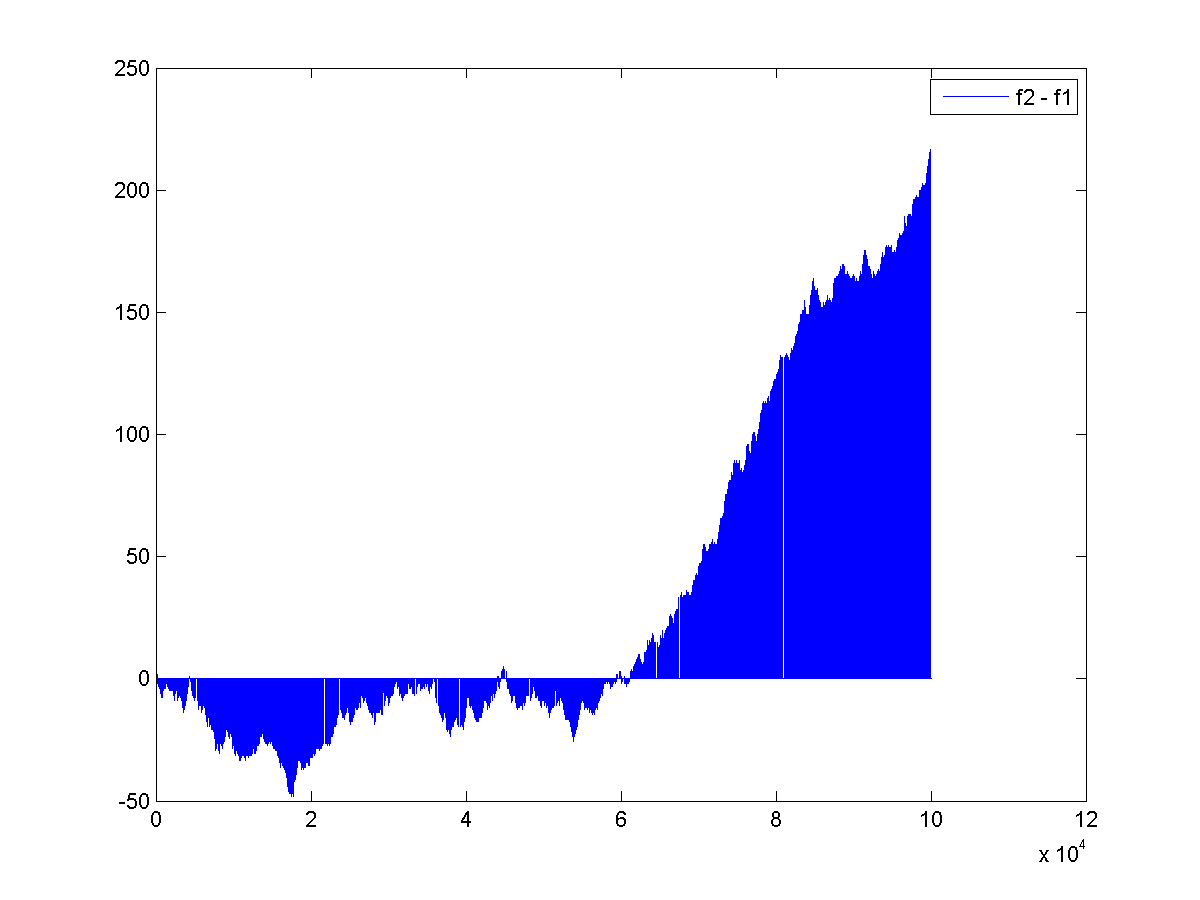
\includegraphics[scale=0.33]{Figures/base1/base4_2} \\
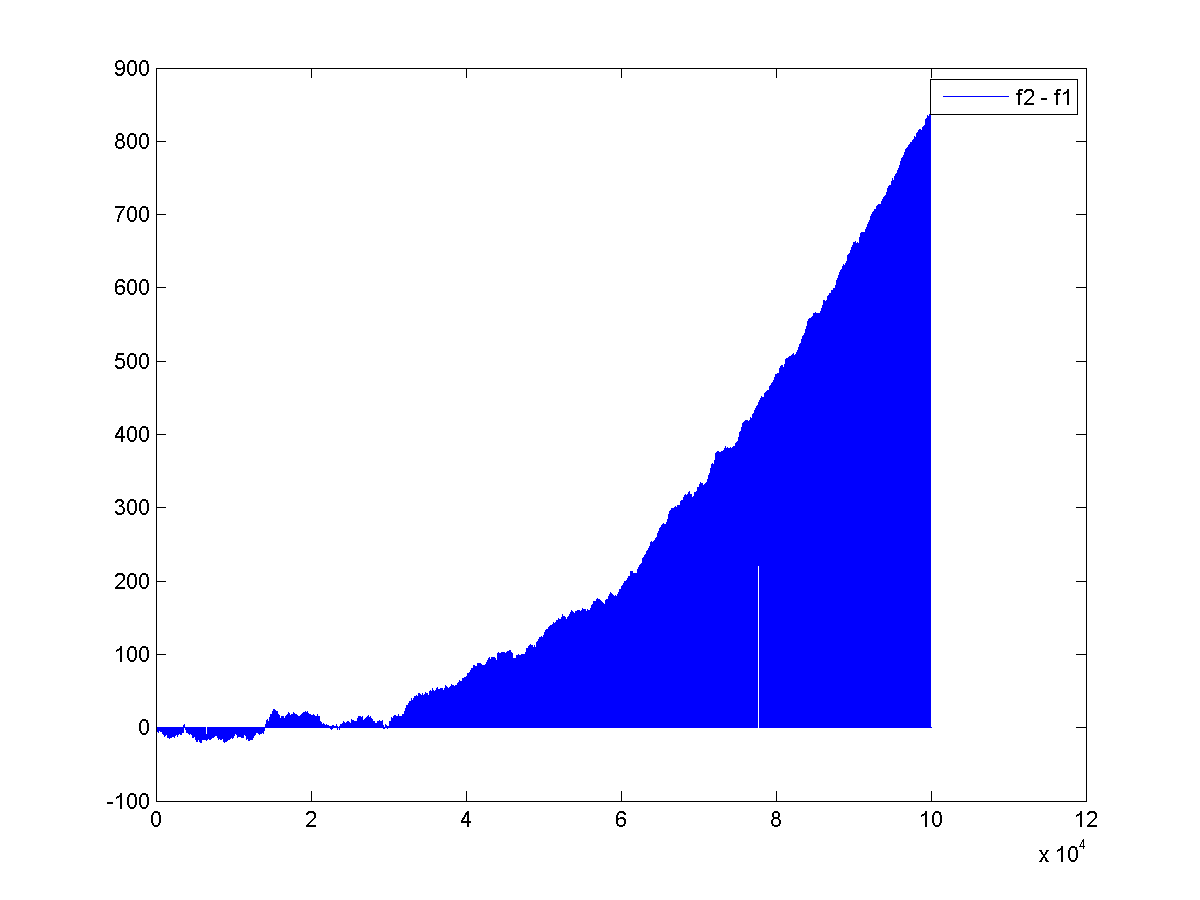
\includegraphics[scale=0.33]{Figures/base1/base4_3}
\end{array}$
\end{center}
\caption[Base case 4]{Results from three simulations for base case 4.}
\label{fig:base4}
\end{figure}

\begin{figure}
\begin{center}$
\begin{array}{ccc}
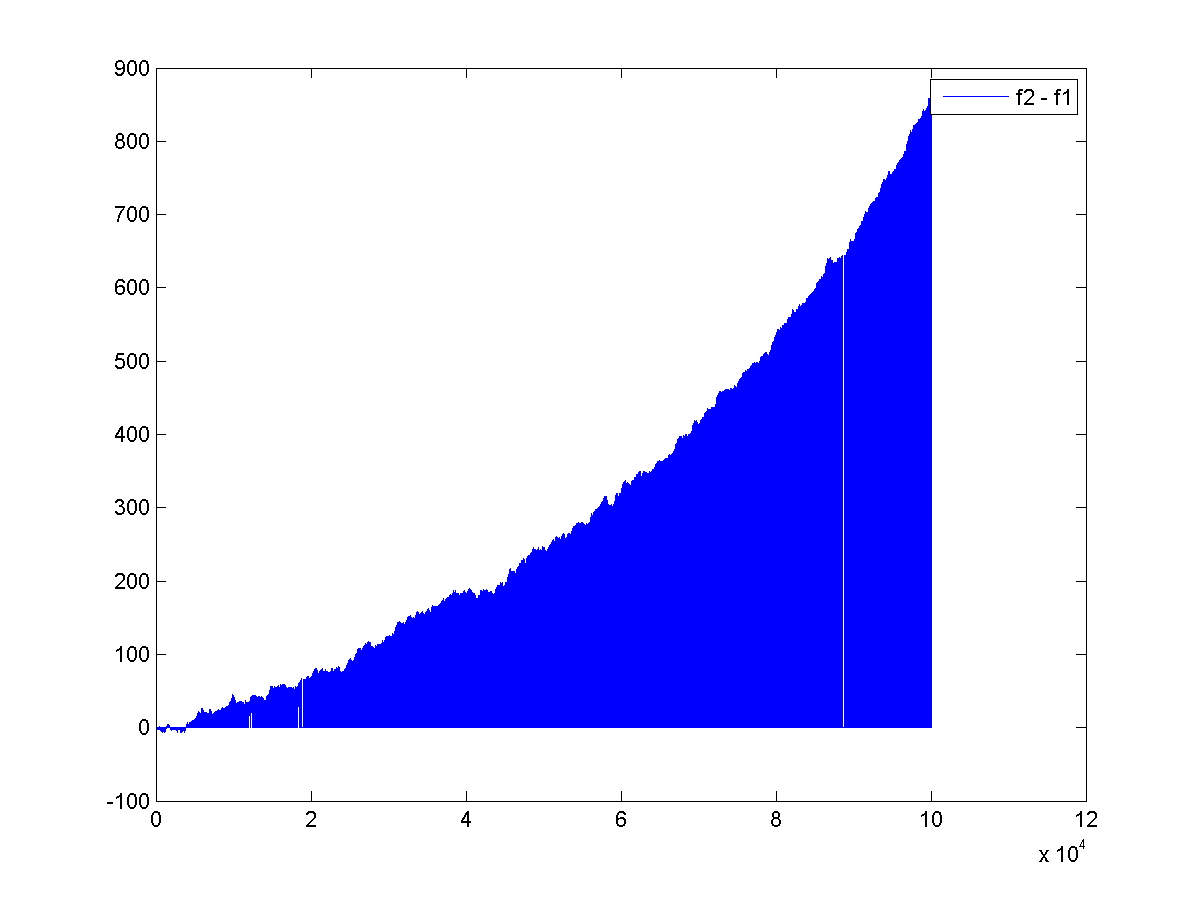
\includegraphics[scale=0.33]{Figures/base1/diff1_1} 
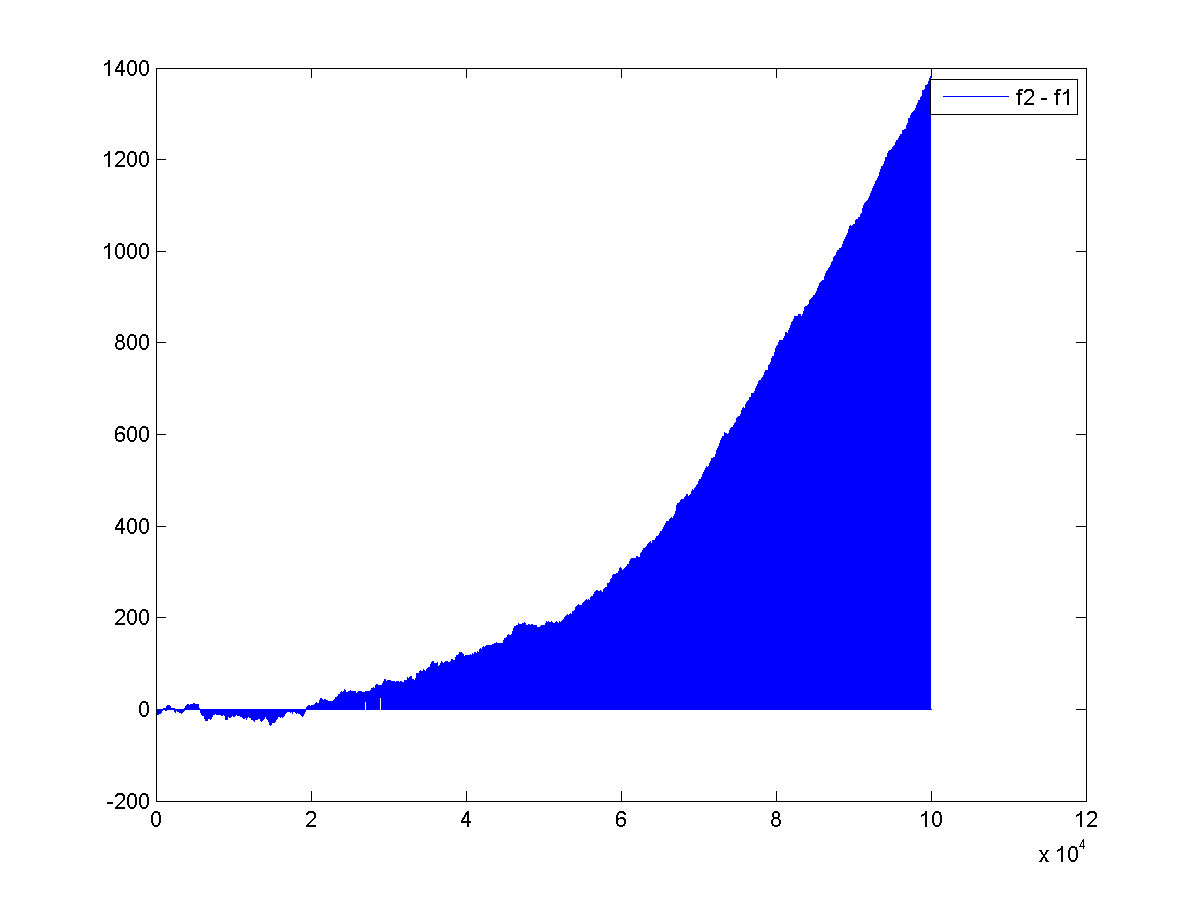
\includegraphics[scale=0.33]{Figures/base1/diff1_2} \\
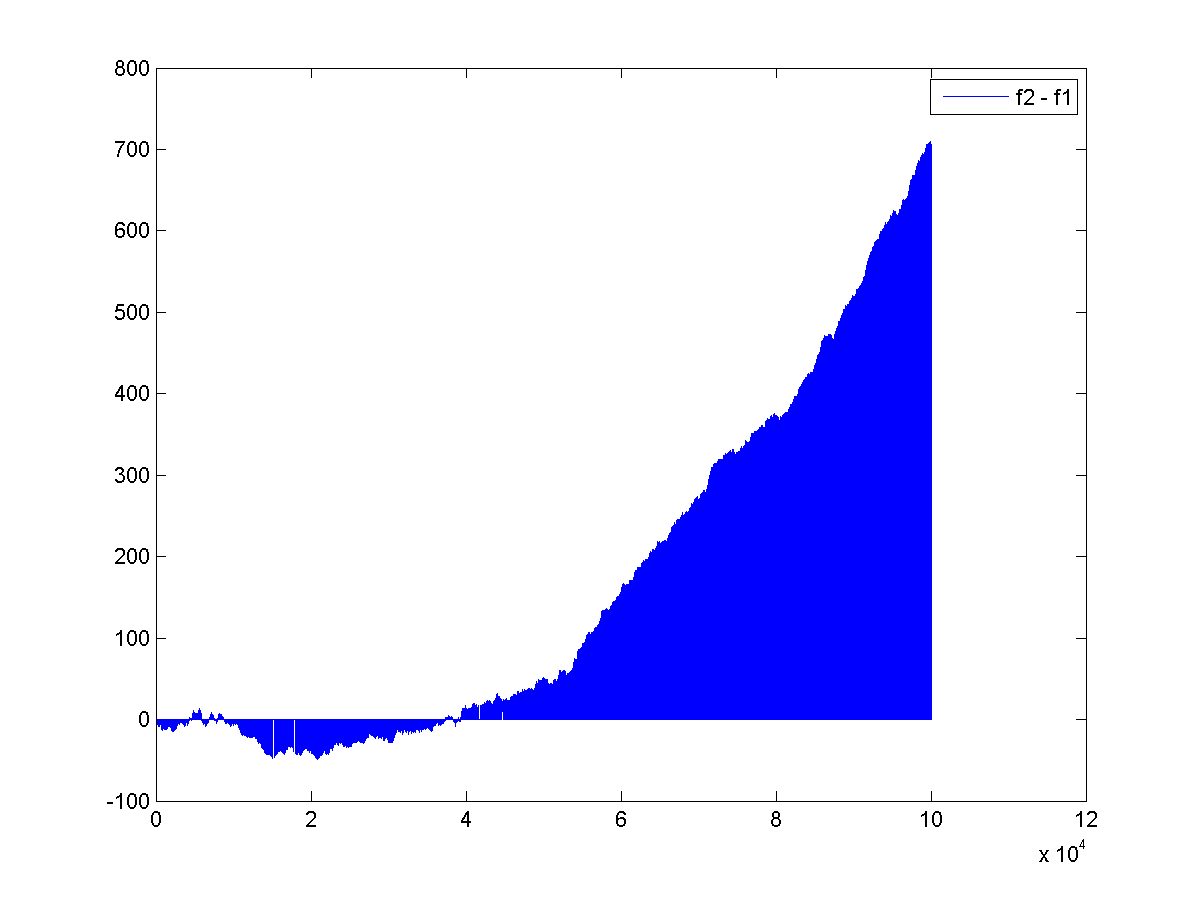
\includegraphics[scale=0.33]{Figures/base1/diff1_3}
\end{array}$
\end{center}
\caption[Difference case 1]{Results from three simulations for difference case 1.}
\label{fig:diff1}
\end{figure}

\begin{figure}
\begin{center}$
\begin{array}{ccc}
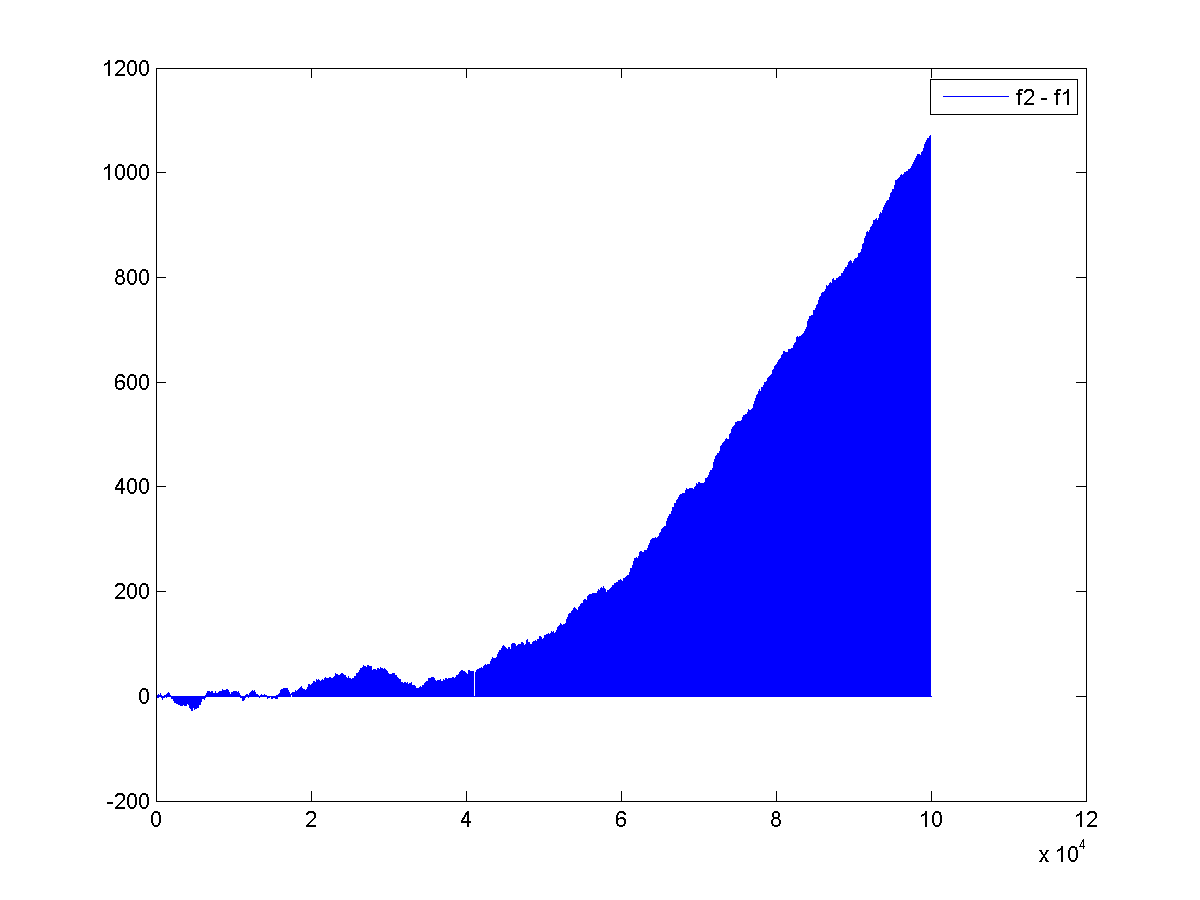
\includegraphics[scale=0.33]{Figures/base1/diff2_1} 
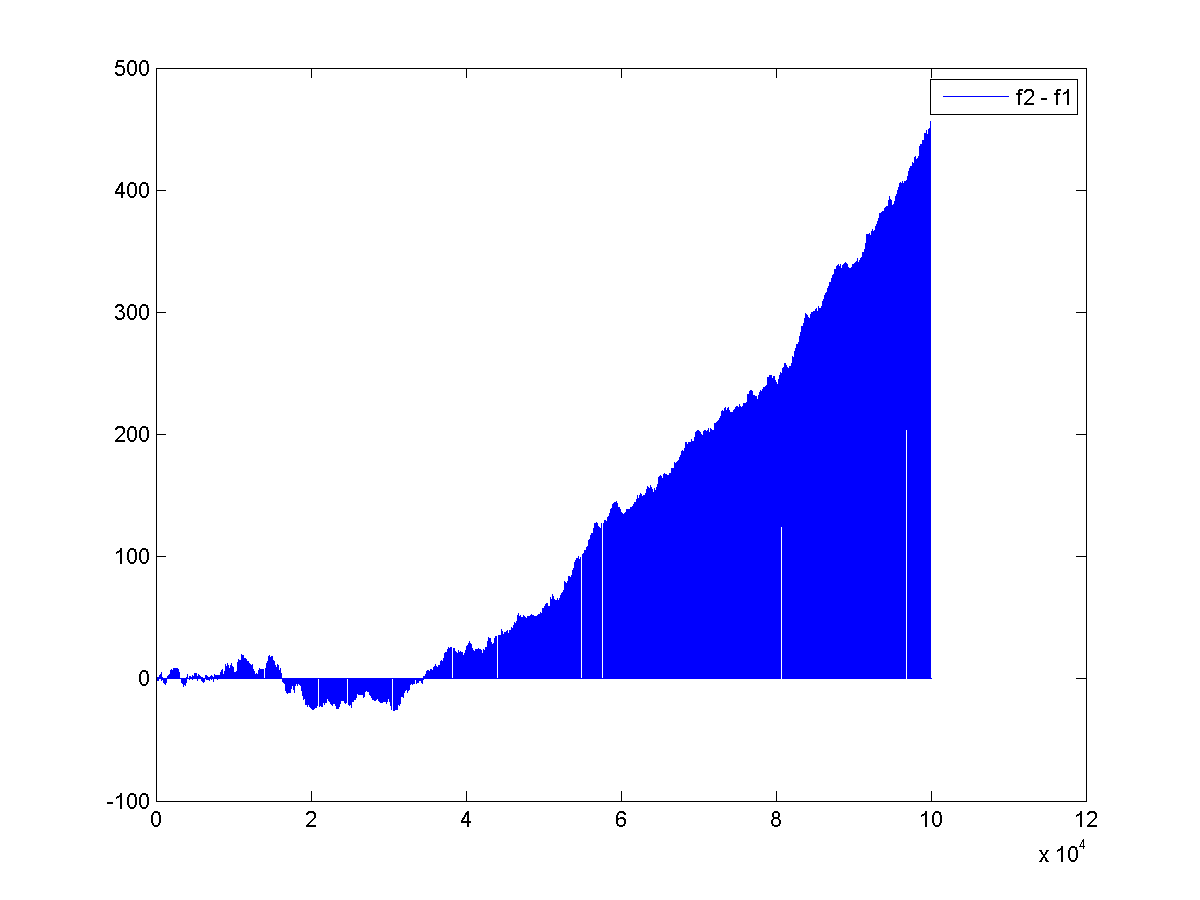
\includegraphics[scale=0.33]{Figures/base1/diff2_2} \\
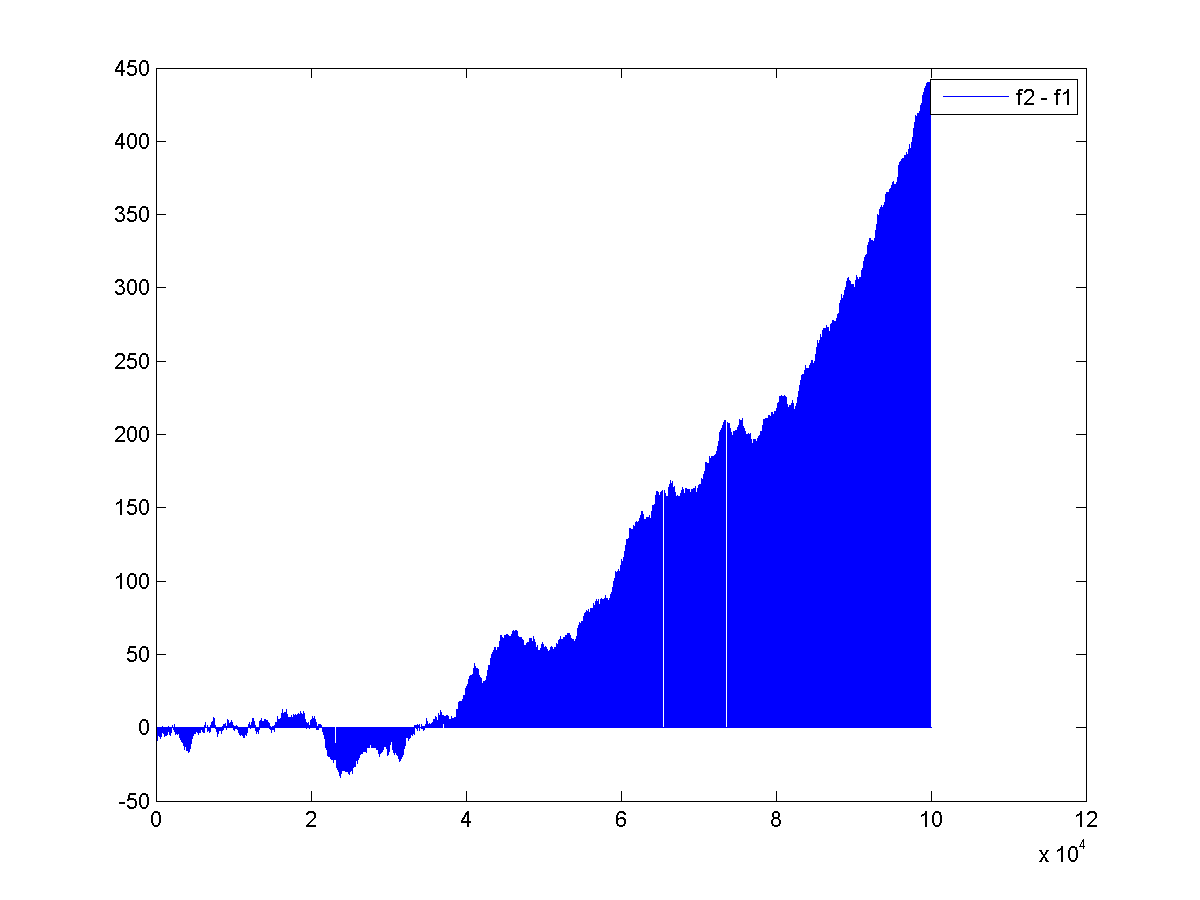
\includegraphics[scale=0.33]{Figures/base1/diff2_3}
\end{array}$
\end{center}
\caption[Difference case 2]{Results from three simulations for difference case 2.}
\label{fig:diff2}
\end{figure}

\begin{figure}
\begin{center}$
\begin{array}{ccc}
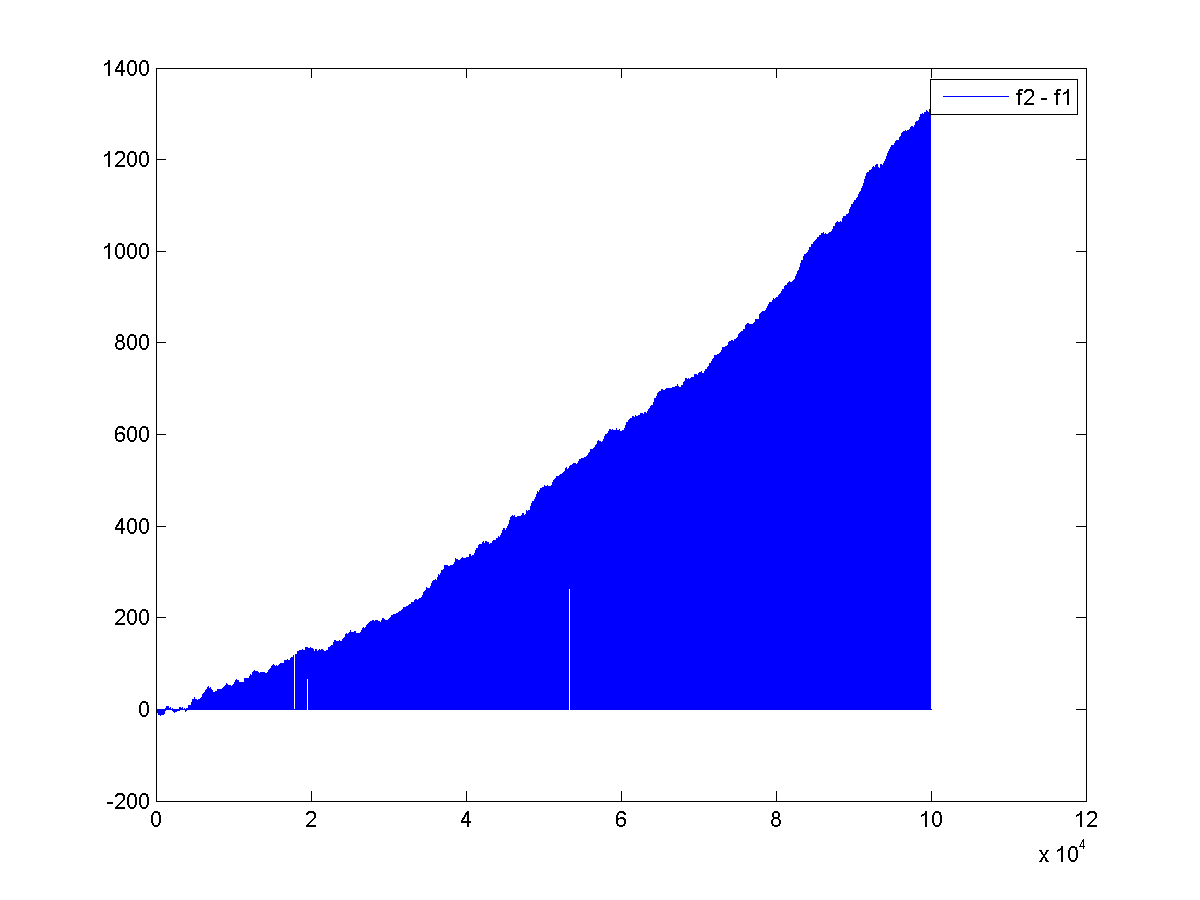
\includegraphics[scale=0.33]{Figures/base1/diff3_1} 
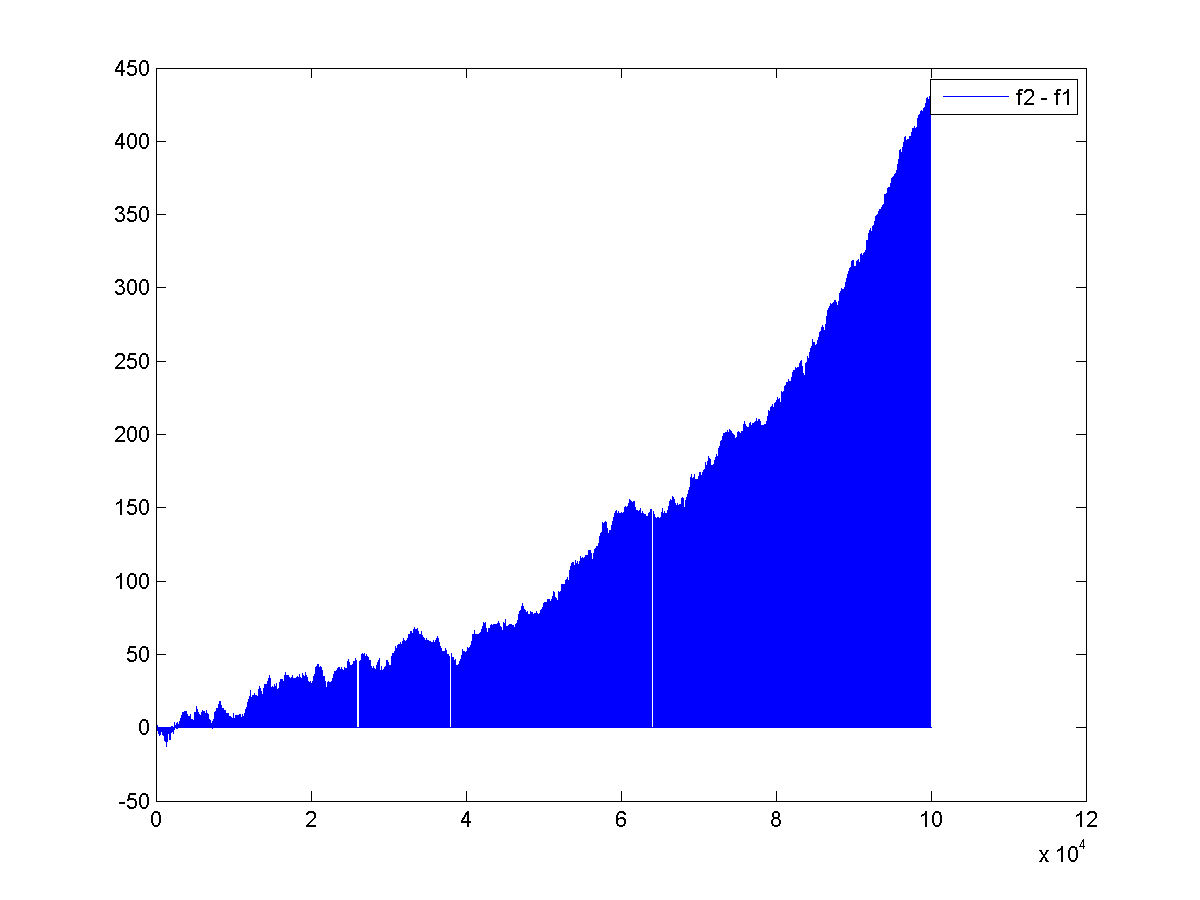
\includegraphics[scale=0.33]{Figures/base1/diff3_2} \\
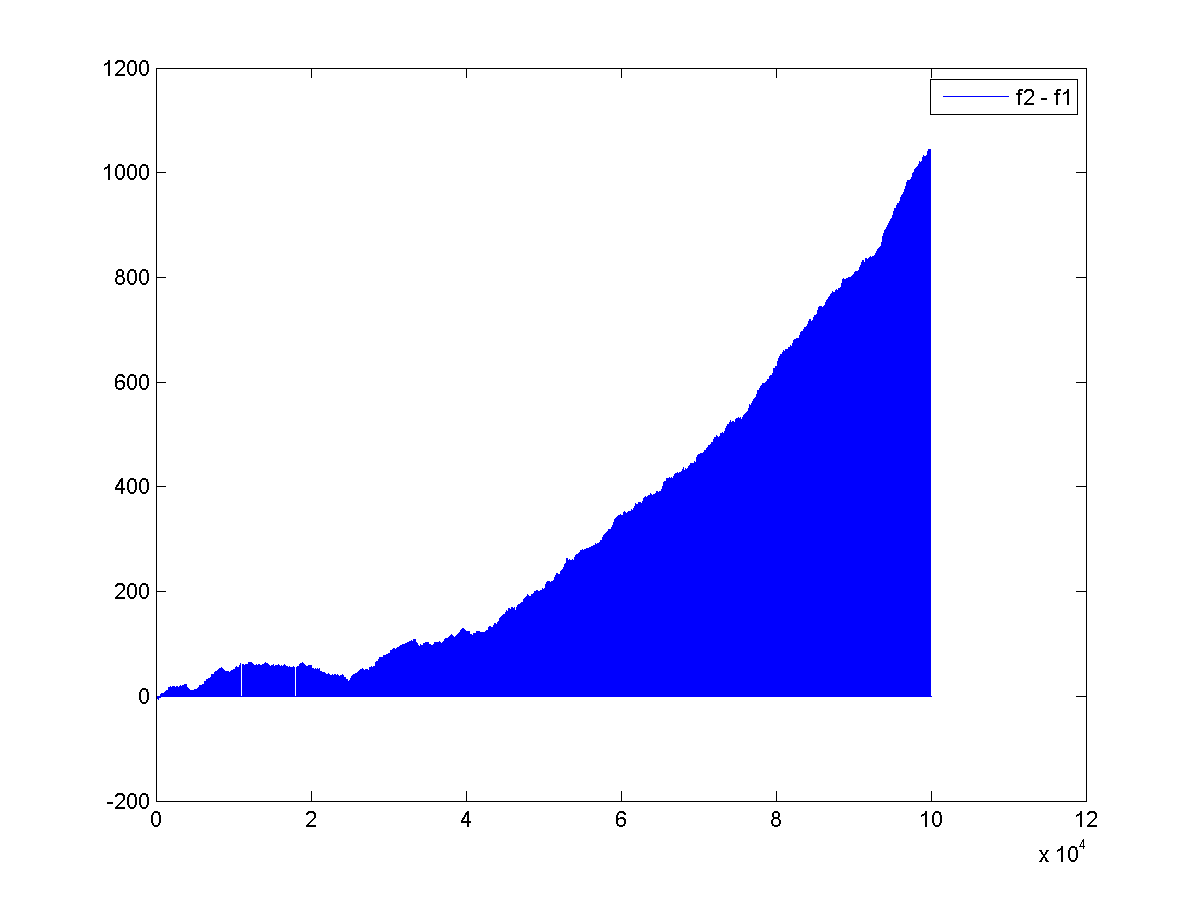
\includegraphics[scale=0.33]{Figures/base1/diff3_3}
\end{array}$
\end{center}
\caption[Difference case 3]{Results from three simulations for difference case 3.}
\label{fig:diff3}
\end{figure}

\begin{figure}
\begin{center}$
\begin{array}{ccc}
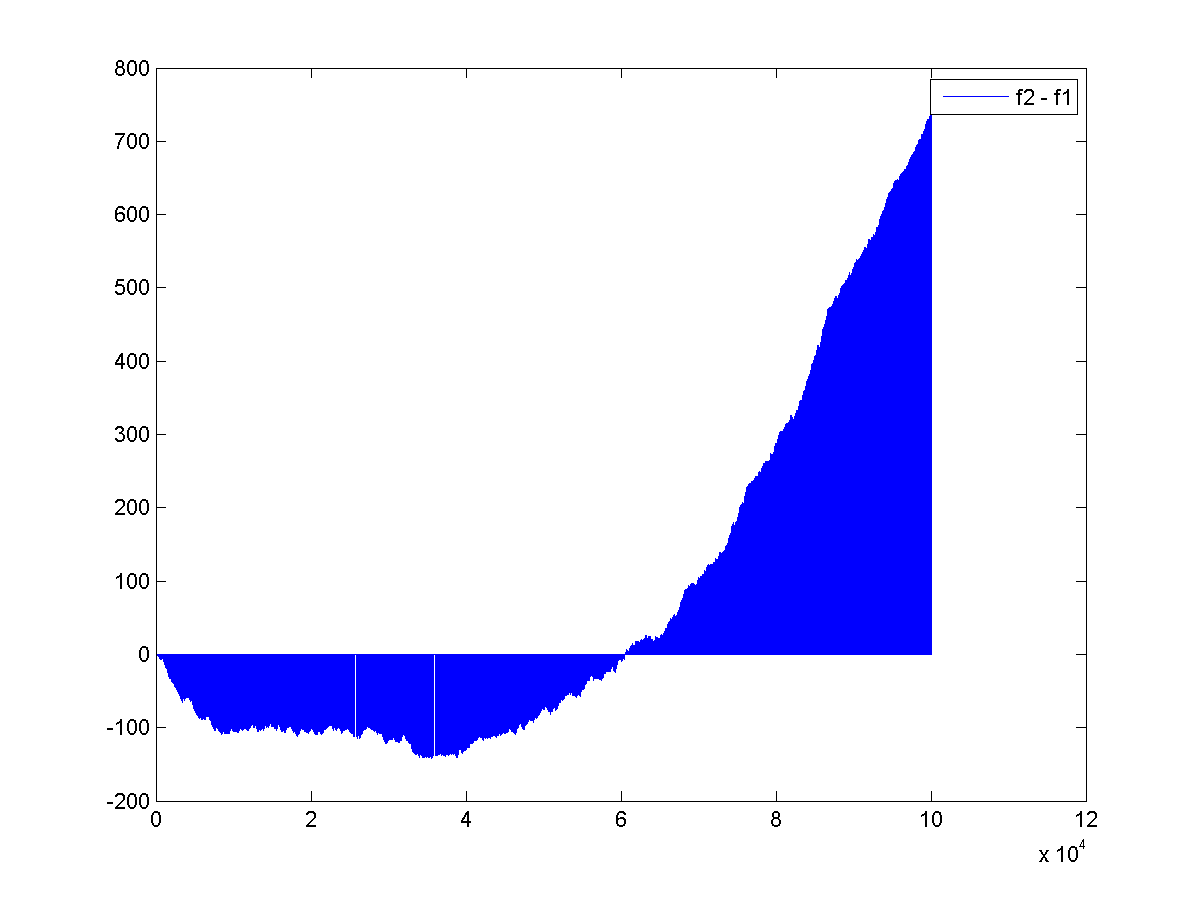
\includegraphics[scale=0.33]{Figures/base1/diff4_1} 
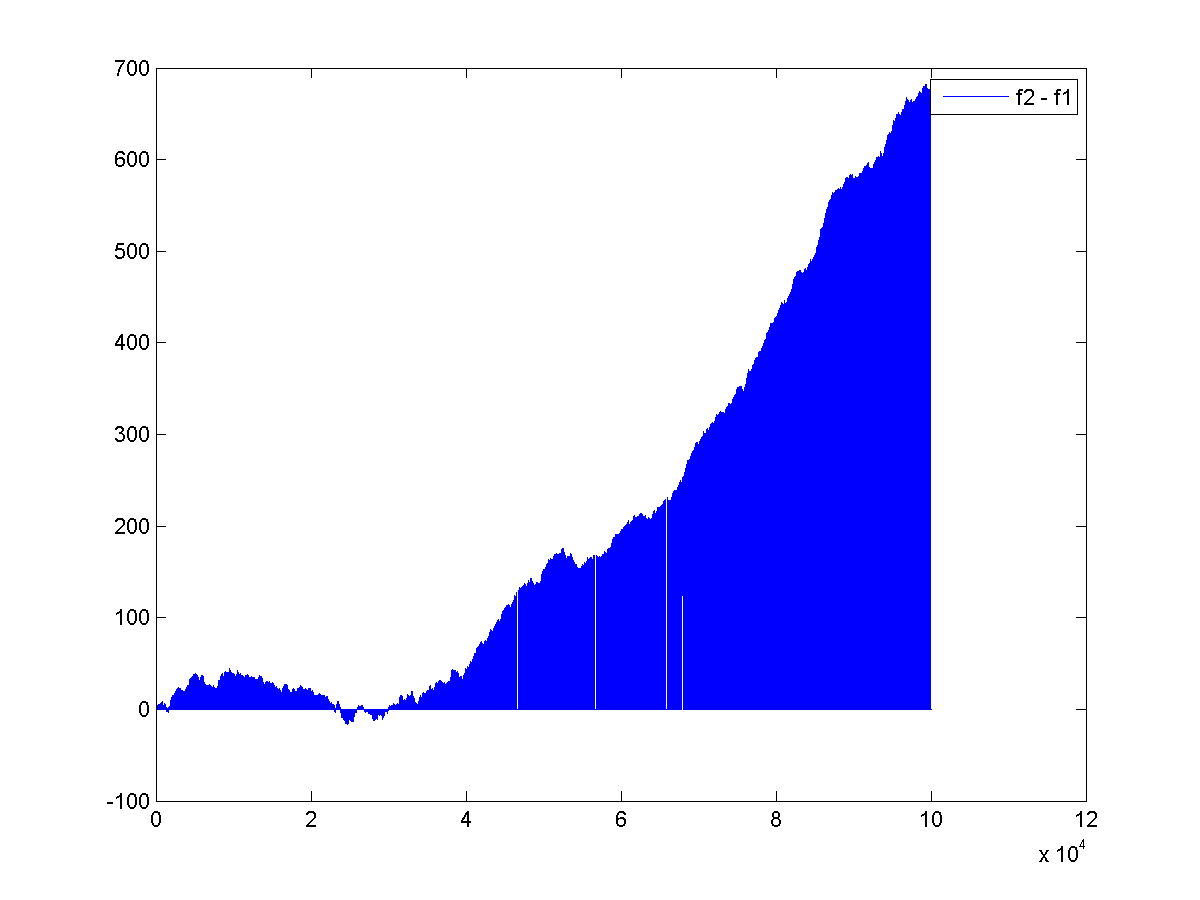
\includegraphics[scale=0.33]{Figures/base1/diff4_2} \\
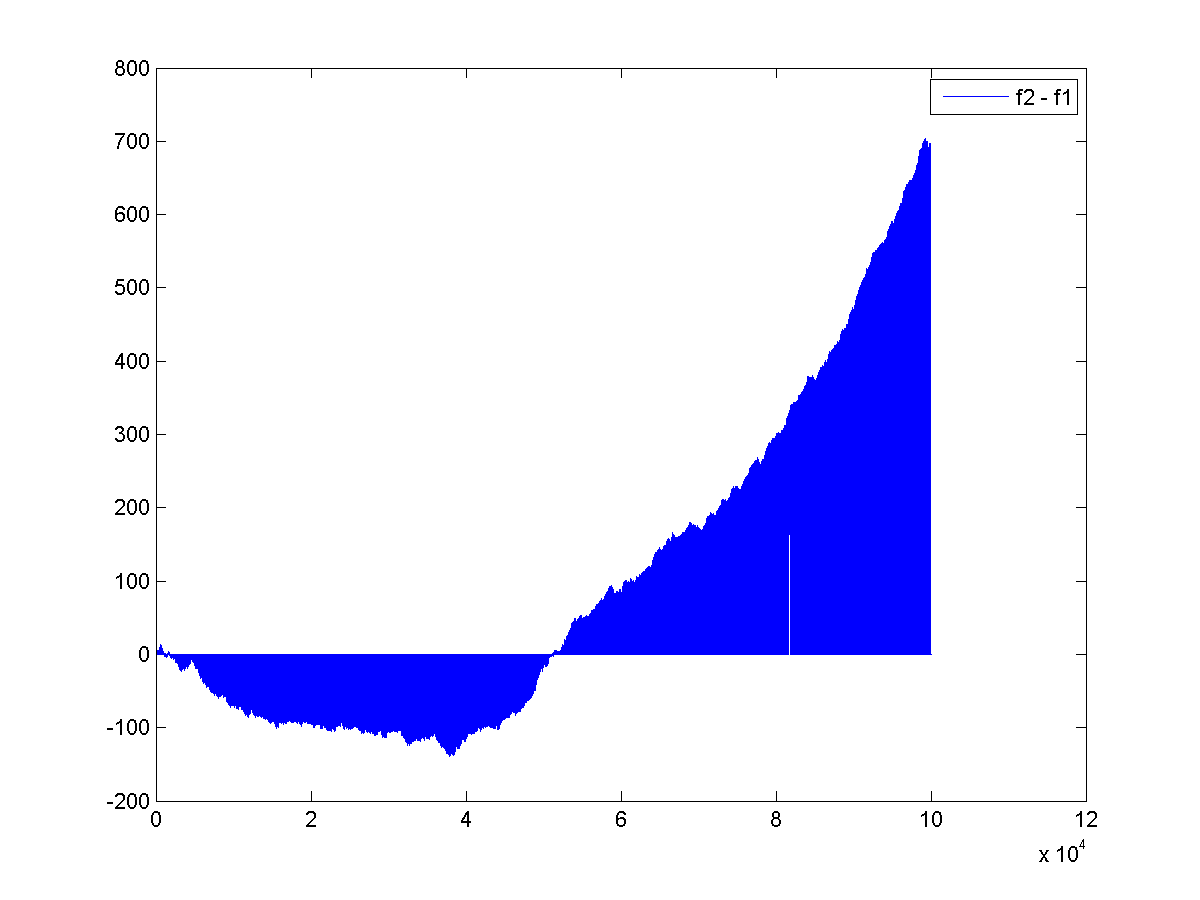
\includegraphics[scale=0.33]{Figures/base1/diff4_3}
\end{array}$
\end{center}
\caption[Difference case 4]{Results from three simulations for difference case 4.}
\label{fig:diff4}
\end{figure}

\begin{figure}
\begin{center}$
\begin{array}{ccc}
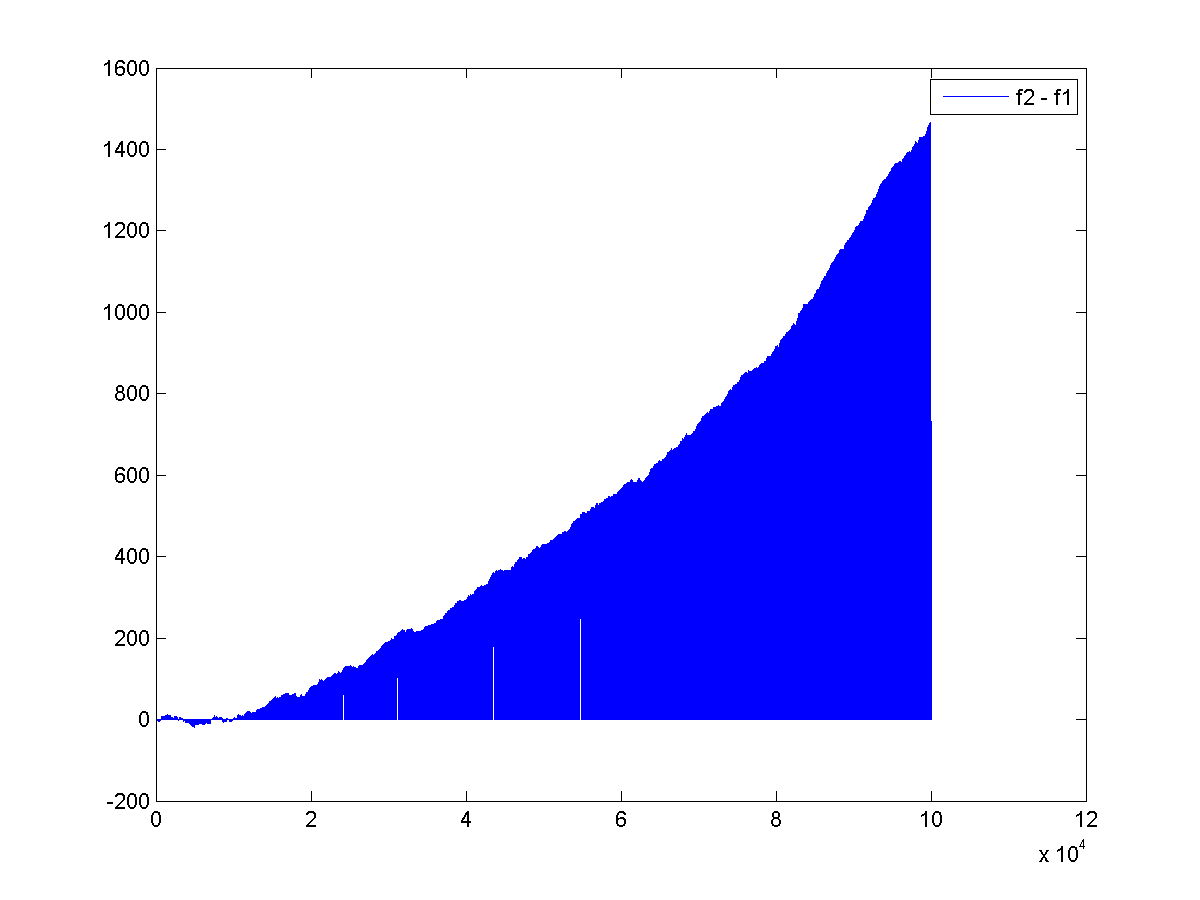
\includegraphics[scale=0.33]{Figures/base1/diff5_1} 
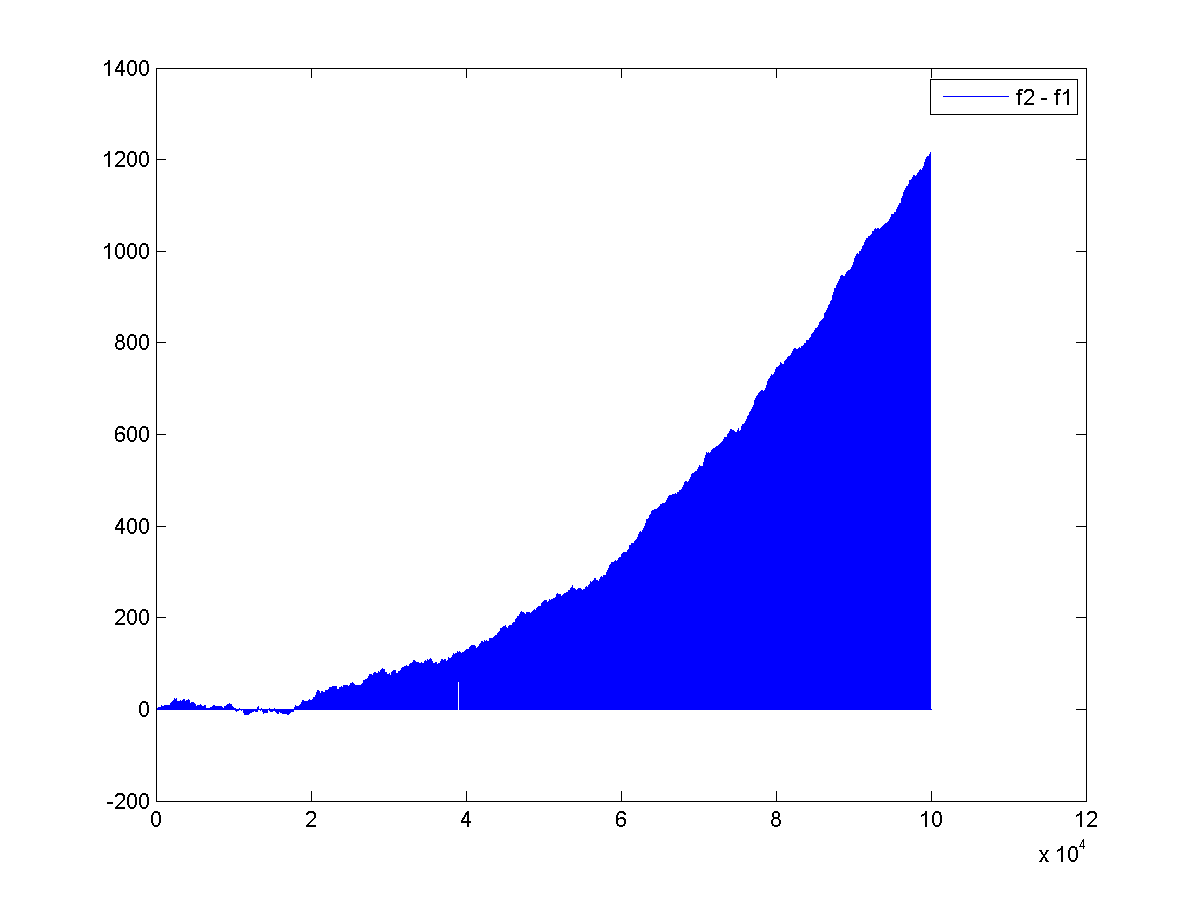
\includegraphics[scale=0.33]{Figures/base1/diff5_2} \\
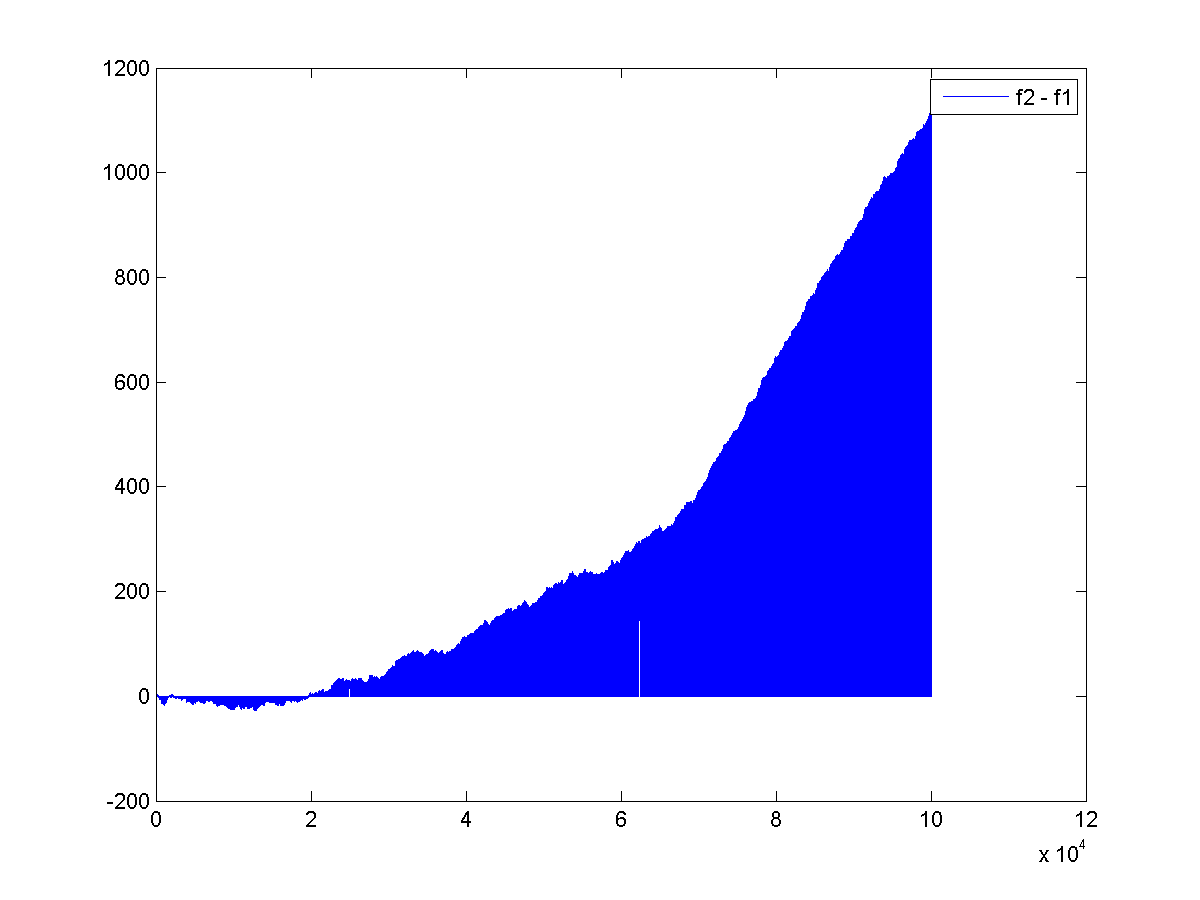
\includegraphics[scale=0.33]{Figures/base1/diff5_3}
\end{array}$
\end{center}
\caption[Difference case 5]{Results from three simulations for difference case 5.}
\label{fig:diff5}
\end{figure}

\begin{figure}
\begin{center}$
\begin{array}{ccc}
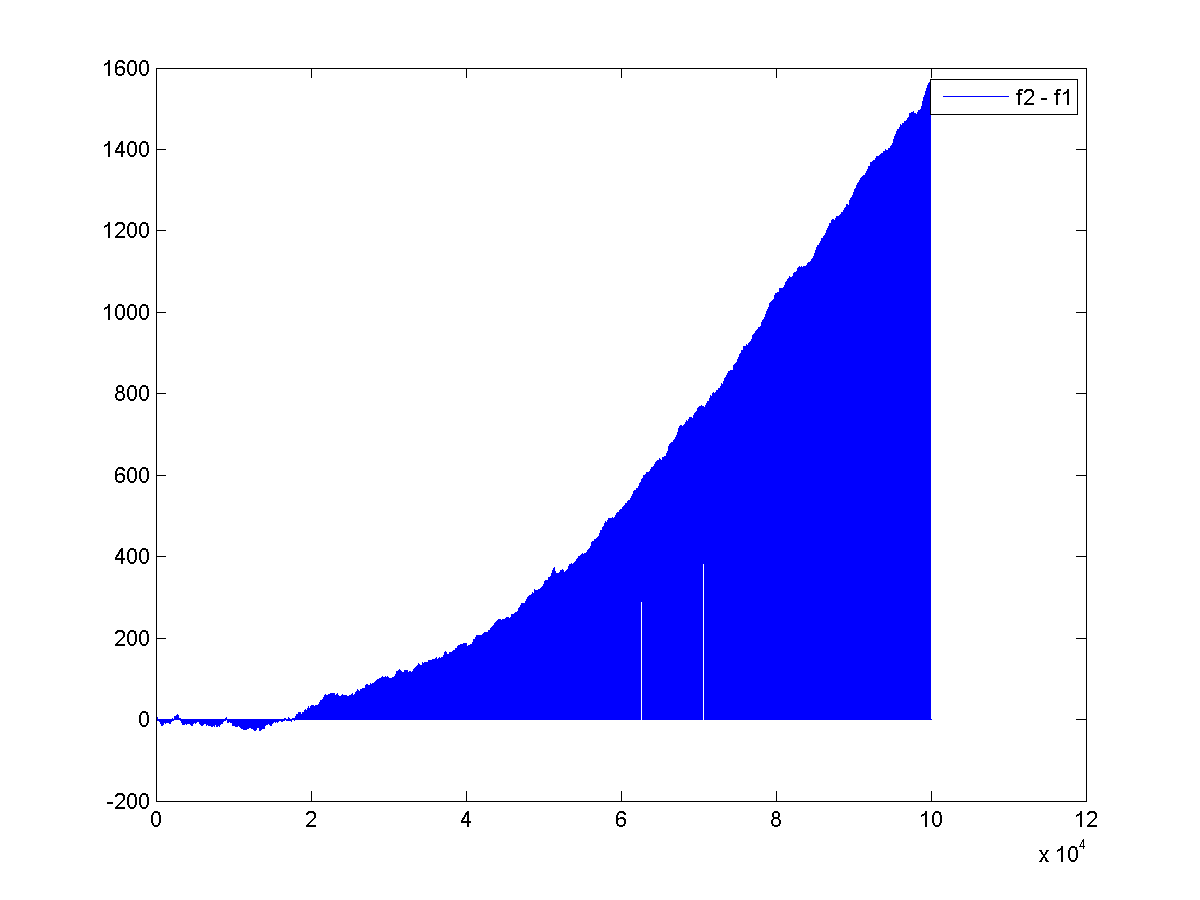
\includegraphics[scale=0.33]{Figures/base1/diff6_1} 
\includegraphics[scale=0.33]{Figures/base1/diff6_2} \\
\includegraphics[scale=0.33]{Figures/base1/diff6_3}
\end{array}$
\end{center}
\caption[Difference case 6]{Results from three simulations for difference case 6.}
\label{fig:diff6}
\end{figure} 
% Chapter Template

\chapter{Significance of Results} % Main chapter title

\label{Chapter5} % Change X to a consecutive number; for referencing this chapter elsewhere, use \ref{ChapterX}

\lhead{Chapter 5. \emph{Significance of Results}} % Change X to a consecutive number; this is for the header on each page - perhaps a shortened title

%----------------------------------------------------------------------------------------
%	SECTION 1
%----------------------------------------------------------------------------------------

\section{The Model}
The model shows us a fast and easy way to generate a scale-free network, and the effects of using the constraint of `likemindedness', defined in chapter~\ref{Chapter3} section~\ref{sec:definitions}, between the agents, which reduces the number of connections formed significantly, while the network still follows power law.

Although this thesis is focused on companies, the modularity of the project allows the algorithm~\ref{alg1} to be used for generic simulation of social structures.

%----------------------------------------------------------------------------------------
%	SECTION 2
%----------------------------------------------------------------------------------------

\section{The Simulation}

The initial results for diffusion in a scale-free network present a picture where it is clear that the spread, whether it is increase or decrease, tends to be exponential. 

The simulation results presented in chapter~\ref{Chapter4} section~\ref{sec:cost_gain} give a varied picture. They are divided into two groups.

%-----------------------------------
%	SUBSECTION 1
%-----------------------------------
\subsection{Base Group}

This group focuses on analysis while cost is same for both companies, and helps the observer to understand the basic nature of the companies. 

The base group analyses show that company2 seems to emerge victor for overall simulation, however, the nature is unstable for shorter runs, i.e., during the initial time steps of the simulations.

The results also suggest that increasing the cost results in more relative profit for Company1. It can be seen that the area under the curve suggesting the net relative gain for Company1 tends to increase as the cost is increased. 


%-----------------------------------
%	SUBSECTION 2
%-----------------------------------

\subsection{Difference Group}

This group focuses on analysis while cost is different for both companies, and allows for analysis of the different policies.

The author focused on two types of policies described in chapter~\ref{Chapter2} section~\ref{sec:policies}. Specifically, the chosen policies were :

\begin{enumerate}
\item[Company1 :] Symbolic involvement. User input is requested but ignored.
\item[Company2 :] Involvement by doing. A user as design team member or as the official liaison with the information system’s development group.
\end{enumerate}


Company1 maintained a minimal involvement of customers in decision making, and made very little effort. This made sure that the company did not take a very high cost. 

Company2 had a more open policy where customers were highly involved, and the company made a lot of significant efforts to reach out. This resulted in formation of long-lasting relations which led to profit in the long run.

The analyses show that company1, with its minimal inclusion policy, is more effective for short-term projects, when it makes less efforts towards the customers. The policy followed by Company2 is less profitable during this phase, but it compensates later on and becomes more profitable than Company1.

The exact shift point for this change is case dependant, and it varies with the value of gain, and cost. But this model could be further developed to prepare prediction system that helps companies to switch between policies in order to maximize their cost-benefit ratio.
 
% Chapter Template

\chapter{Extending the Analysis} % Main chapter title

\label{Chapter6} % Change X to a consecutive number; for referencing this chapter elsewhere, use \ref{ChapterX}

\lhead{Chapter 6. \emph{Extending the Analysis}} % Change X to a consecutive number; this is for the header on each page - perhaps a shortened title

The present system is focused on only two companies, competing over a single attribute of the agent. It is limited to a specific  part of a very wide spectra of possibilities.

In future, there are possibilities to extend this sytem and anlyse a diversity of scenarios.

%----------------------------------------------------------------------------------------
%	SECTION 1
%----------------------------------------------------------------------------------------

\section{Extending the analysis to more companies}

The environment could always include more companies competing for the same slot. This might provide valuable insight, specially for cases where two companies might collaborate for mutual benefit against a common competing company.

%----------------------------------------------------------------------------------------
%	SECTION 2
%----------------------------------------------------------------------------------------

\section{Extending the analysis to more attributes}

The companies in the present model only compete for a single attribute, but this may be extended to make them compete for multiple attributes of the  agents. However, this will significantly increase the complexity if the model.

%----------------------------------------------------------------------------------------
%	SECTION 3
%----------------------------------------------------------------------------------------

\section{Extending the analysis to collaborative diffusion over single attribute or multiple attributes}

While the presented system only lets the companies compete against each other, it might be interesting to see how they behave when they are collaborating towards a common goal. This could be done for a single attribute as well as multiple attributes. 
%----------------------------------------------------------------------------------------
%	SECTION 4
%----------------------------------------------------------------------------------------

\section{Extending to Other Systems}

The present system is targeted towards company policies, but the generic nature and social structure of the model imparts flexibility to the system which makes it easy to extend it to other systems as well. 
% Chapter Template

\chapter{Summary and Conclusion} % Main chapter title

\label{Chapter7} % Change X to a consecutive number; for referencing this chapter elsewhere, use \ref{ChapterX}

\lhead{Chapter 7. \emph{Summary and Conclusion}} % Change X to a consecutive number; this is for the header on each page - perhaps a shortened title

In this thesis, the author presents methods to create a scale-free network fir for his purpose by following a slightly modified form~\ref{alg1} of the B-A Algorithm, and then he goes on to simulate an environment where two companies are competing to win over the agents in the network.
He uses the data gathered to analyse the policies followed by the companies while attracting the customers, and presents his findings which suggest a basic model for maximizing cost to gain ration for the companies.

He also suggests that similar approach could be used in wearable tech to let devices connect and map the social structure of their users, and this model would provide analytical ability over such a network.

 

%----------------------------------------------------------------------------------------
%	THESIS CONTENT - APPENDICES
%----------------------------------------------------------------------------------------

\addtocontents{toc}{\vspace{2em}} % Add a gap in the Contents, for aesthetics

\appendix % Cue to tell LaTeX that the following 'chapters' are Appendices

% Include the appendices of the thesis as separate files from the Appendices folder
% Uncomment the lines as you write the Appendices

% Appendix A

\chapter{Appendix Title Here} % Main appendix title

\label{AppendixA} % For referencing this appendix elsewhere, use \ref{AppendixA}

\lhead{Appendix A. \emph{Appendix Title Here}} % This is for the header on each page - perhaps a shortened title

Appendix goes here.
%% Appendix Template

\chapter{Barab\'asi Albert Model} % Main appendix title

\label{AppendixB} % Change X to a consecutive letter; for referencing this appendix elsewhere, use \ref{AppendixX}

\lhead{Appendix X. \emph{B-A Model}} % Change X to a consecutive letter; this is for the header on each page - perhaps a shortened title

This algorithm for generating random scale-free networks was developed in 1999.
This model was developed when researching the structure of the World Wide Web and the initial expectations of the researchers was to find a random network, but instead, they witnessed the existence of Power-Law in the degree distribution of the nodes, and the concept of scale-free networks was born.

This structure explain the presence of a few highly-connected hubs and a larger number of less connected nodes in the networks, and the architecture holds true for a wide range of networked structures, varying from a man-made physical infrastructures like the internet to the biological networks of proteins.

This model also emphasises on the role of hubs, which is very important and have applications in fields ranging from IT security to spread of contagious diseases and more. In words of Albert-L\'aszl\'o Barab\'asi, the hubs make the scale-free networks ``very robust to random failures, but very fragile to targeted attacks". 

%\input{Appendices/AppendixC}

\addtocontents{toc}{\vspace{2em}} % Add a gap in the Contents, for aesthetics

\backmatter

%----------------------------------------------------------------------------------------
%	BIBLIOGRAPHY
%----------------------------------------------------------------------------------------

\label{Bibliography}

\lhead{\emph{Bibliography}} % Change the page header to say "Bibliography"

\bibliographystyle{unsrtnat} % Use the "unsrtnat" BibTeX style for formatting the Bibliography

\bibliography{Bibliography} % The references (bibliography) information are stored in the file named "Bibliography.bib"

\end{document}  